\documentclass[a4paper,12pt]{book}

\usepackage[polish]{babel}
\usepackage[utf8]{inputenc}
\usepackage[OT4]{fontenc}
\usepackage{tabularx}
\usepackage{geometry}
\usepackage[pdftex]{graphicx}
\usepackage[T1]{fontenc}
\usepackage{listings}
\usepackage{subfigure}
\usepackage{url}

\geometry{verbose,a4paper,tmargin=2.5cm,bmargin=2.5cm,lmargin=3cm,rmargin=2.5cm}

\linespread{1.5}

\pagestyle{empty}

\author{Jakub Odias}
\title{Konstrukcja platformy sprzętowej dla potrzeb wbudowanego systemu Linux}

\begin{document}
	{\fontfamily{phv}\selectfont
	\begin{titlepage}
		\vspace*{15pt}
		\begin{figure}[htp]
			\begin{center}
				
\includegraphics[scale=0.25]{img/polsl.png}
			\end{center}
		\end{figure}

		\vspace{-9pt}
		\begin{center}
			
			\Large{\textbf{P}}\large{\textbf{OLITECHNIKA}}\Large{\textbf{ Ś}}\large{\textbf{LĄSKA}}\\

			\vspace{10pt}
			
			\Large{\textbf{W}}\large{\textbf{YDZIAŁ }}\Large{\textbf{A}}\large{\textbf{UTOMATYKI, }}\Large{\textbf{E}}\large{\textbf{LEKTRONIKI I }}\Large{\textbf{I}}\large{\textbf{NFORMATYKI}}\\

			\vspace{75pt}
			
			\Large{Praca dyplomowa magisterska}
			
			\vspace{38pt}
			
			\large{Konstrukcja platformy sprzętowej dla potrzeb \\wbudowanego systemu Linux}
		\end{center}
		\vspace{85pt}
		
		\begin{flushleft}
			\large{Autor: Jakub Odias}\\
			\vspace{5pt}
			\large{Kierujący pracą: dr inż. Krzysztof Tokarz}\\

			\vspace{105pt}
			\normalsize{Gliwice, sierpień 2009}
		\end{flushleft}
	\end{titlepage}}

	\tableofcontents

	\pagestyle{plain}
	
%------------------------------------------------------------------------------------
% WSTĘP
%------------------------------------------------------------------------------------

	\chapter{Wstęp}
		\section{Wprowadzenie}
			Wraz z rozwojem informatyki pojawia się coraz więcej układów sprzętowych, różnorodnych protokołów oraz użytecznych aplikacji i bibliotek. Aby napisać sterownik urządzenia lub programową obsługę dla danego protokołu, należy zazwyczaj poświęcić dużo czasu i zasobów na zapoznanie się z dokumentacją, napisanie programu oraz wystarczające przetestowanie.\\
			Dlatego podczas tworzenia zaawansowanego układu sprzętowego, wygodnym rozwiązaniem jest użycie gotowego i stabilnego kodu, który obsłuży większość potrzebnych użytkownikowi funkcjonalności. Firmy zajmujące się produkcją nowych urządzeń, np. telefonów komórkowych czy routerów bezprzewodowych, zazwyczaj wykorzystują rozwijane przez siebie aplikacje lub proste systemy operacyjne w celu przyspieszenia wstępnej fazy uruchamiania nowego oprogramowania oraz późniejszego efektywnego zarządzania zasobami. Możliwe jest także zastosowanie gotowych rozwiązań, takich jak zaawansowane systemy operacyjne Windows Embedded i Linux; wadą wbudowanej wersji Windowsa jest niestety to że nie jest to darmowe oprogramowanie, oraz w przeciwieństwie do Linuksa nie posiada ogólnodostępnego kodu źródłowego. Dzięki udostępnieniu plików źródłowych jądra (ang. kernel) systemu Linux na licencji GNU General Public License 2 \cite{website:gnu_gpl_v2}, każdy programista może dla swoich potrzeb napisać sterownik, a następnie udostępnić go innym - w ten sposób dodawanie nowych funkcjonalności oraz poprawianie ewentualnych błędów jest znacznie uproszczone.\\
			Dzięki wiedzy o tym w jaki sposób zaprojektować platformę sprzętową, umożliwiającą uruchomienie systemu operacyjnego na prostym układzie mikroprocesorowym, można stworzyć urządzenie które ma bardzo rozbudowane możliwości, porównywalne z tymi dostępnymi w urządzeniach przenośnych.
		\section{Cel pracy}
			Celem niniejszej pracy magisterskiej jest konstrukcja platformy sprzętowej dostosowanej do potrzeb wbudowanego systemu Linux (ang. Embedded Linux). Platforma ma mieć mozliwość podłączenia pamięci masowych typu Compact  Flash lub dysk IDE, wyświetlaczy graficznych LCD, urządzeń USB oraz sieci Ethernet.\\
			Głównym zadaniem było zaprojektowanie oraz wykonanie części sprzętowej projektu, spełniającej powyższe wymagania, a następnie zapoznanie się z wbudowaną wersją systemu Linux i jej implementacja na gotowym układzie.\\
		\section{Wbudowany Linux}
			W odróżnieniu od systemu operacyjnego Linux, stosowanego w komputerach domowych lub na serwerach, wbudowana wersja jest przeznaczona dla urządzeń z ograniczonymi zasobami, np. urządzeń mobilnych. Pełnią one ściśle określoną rolę, więc nie muszą zawierać zbędnego lub mało używanego oprogramowania oraz niepotrzebnych sterowników. Dodatkowo mają zazwyczaj ograniczoną ilość pamięci RAM, szybkość pracy procesora oraz niewiele zasobów dyskowych więc ważna jest także odpowiednia konfiguracja i optymalizacja takiego systemu.\\
			Określenie 'Wbudowany Linux' oznacza zatem jedynie konfigurację systemu dla konkretnych potrzeb - jądro Linuksa jest niemal identyczne jak w przypadku komputerów klasy PC lub podobnych.
		\section{Platforma sprzętowa}
			Podczas konstruowania uniwersalnej platformy sprzętowej dla Linuksa istotne jest wzięcie pod uwagę następujących czynników:
			\begin{itemize}
				\item Linux jest systemem 32-bitowym więc procesor użyty w projekcie również powinien mieć architekturę 32-bitową. Co prawda istnieją wersje Linuksa dostosowane dla mikroprocesorów 8- lub 16-bitowych, jednak nie są one dostatecznie wspierane.
				\item System operacyjny Linux wymaga żeby procesor implementował jednostkę zarządzania pamięcią (MMU) w celu efektywnego i bezpiecznego używania pamięci. Istnieje okrojona wersja $\mu$cLinux\cite{website:uclinux} dostosowana do potrzeb mikroprocesorów niewyposażonych w MMU.
				\item Tworzony układ powinien móc wykonać dostateczną liczbę operacji na sekundę oraz mieć ilość pamięci RAM wystarczającą do uruchomienia zaawansowanego systemu operacyjnego.
				\item Platforma powinna umożliwić podłączenie jak najmniejszym kosztem sieci Ethernet, urządzeń USB oraz wszelkich innych układów.
			\end{itemize}
		\section{Przykładowe implementacje}
			Linux jest obecnie najpopularniejszym systemem operacyjnym wśród producentów systemów wbudowanych m.in. telefonów komórkowych, Palmtopów, przełączników i routerów sieciowych oraz systemów przemysłowych.\\
			Podczas projektowania układu pomocne jest wzorowanie się na działających rozwiązaniach, które pełnią podobne funkcje.\\
			W dodatku \ref{app:przykladowe_projekty} znajduje się lista stron WWW mieszczących projekty, z których korzystał autor tej pracy.



%------------------------------------------------------------------------------------
% CZĘŚĆ SPRZĘTOWA
%------------------------------------------------------------------------------------

	\chapter{Część sprzętowa}
		\section{Wprowadzenie}
			W tej części zostanie przedstawiony dobór, wraz z objaśnieniem, wszystkich układów sprzętowych użytych w projekcie oraz opis zagadnień na które należało zwracać uwagę podczas projektowania platformy.\\
			W dodatku \ref{app:gotowy_projekt} znajdują się schematy i zdjęcia zaprojektowanego układu.
		\section{Mikroprocesor}
			\subsection{Wymagania}
				Podczas wyboru mikroprocesora, który będzie stanowił rdzeń platformy, kierowano się tym aby wybrany układ scalony posiadał następujące cechy:
				\begin{itemize}
					\item architektura 32-bitowa
					\item jednostka zarządzania pamięcią MMU
					\item maksymalna szybkość pracy mikroprocesora wystarczająca do efektywnego działania systemu operacyjnego
					\item sprzętowa obsługa portów USB i Ethernet
					\item interfejs SPI i/lub MMC w celu podłączenia kart pamięci SD/MMC
					\item wbudowany kontroler pamięci SDRAM
					\item dostępność układu w obudowie umożliwiającej stosunkowo łatwe przylutowanie np. TQFP
				\end{itemize}
			\subsection{Porównanie dostępnych układów}
				Na rynku jest dostępnych wiele procesorów o architekturach spełniających wymagania projektu m.in. x86, PowerPC, MIPS, ARM i AVR32, jednak jedynie 2 ostatnie z nich są łatwo dostępne w ilościach detalicznych.\\
				Zarówno ARM jak i AVR32 są wspierane przez jądro systemu Linux, jednak kod dla 32-bitowej architektury mikrokontrolerów AVR został udostępniony stosunkowo niedawno, bo dopiero w wersji 2.6.19. W związku z tym zdecydowano się na wykorzystanie jednego z procesorów zawierających rdzeń firmy ARM\cite{website:arm}, które już od dłuższego czasu posiadają stabilne sterowniki w źródłach kernela.\\
				Układy oparte o rdzenie ARM są produkowane przez różne firmy np. Philips zajmuje się wytwarzaniem mikrokontrolerów ARM7TDMI, niestety nie są one wyposażone w jednostkę MMU, natomiast firma Atmel jest uznanym producentem układów m.in. z rodzin ARM9TDMI i ARM9E. Mikroprocesory z nowszymi rdzeniami, takimi jak XScale i Cortex, są trudno dostępne do zakupu oraz występują zazwyczaj w obudowach BGA.\\
				Po zapoznaniu z ofertą firmy Atmel, okazało się że jedynie mikrokontrolery AT91RM9200 i AT91SAM9260 spełniają wymagania projektu (są dostępne w Polsce oraz występują w obudowach QFP208). W tabeli \ref{tab:arm_comparison} znajduje się porównanie najważniejszych cech obu układów.
				
				\begin{table}[]
					%\extrarowheight=3pt
					\begin{tabularx}{\textwidth }{|c|X|X|}
						\hline \textbf{Cecha} &\textbf{AT91RM9200} & \textbf{AT91SAM9260} \\ 
						\hline Rdzeń & ARM920T & ARM926EJ-S - rozszerzone rozkazy DSP, technologia ARM Jazelle\textsuperscript{\textregistered} dla Javy \\
						\hline Szybkość & 200 MIPS @ 180 MHz & 200 MIPS @ 180 MHz \\
							procesora & & \\
						\hline Pamięć cache & 16kB dane, 16kB instrukcje & 8kB dane i 8kB instrukcje \\
						\hline Wbudowana pamięć & 16kB SRAM, 128kB ROM & 4kB SRAM, 32 kB ROM \\
						\hline Ethernet & kontroler MAC 10/100T z interfejsem MII & kontroler MAC 10/100T z interfejsem MII \\
						\hline USB & USB 2.0 - tryb urządzenia i gospodarza & USB 2.0 - tryb urządzenia i gospodarza \\
						\hline Możliwość podłączenia & SDRAM, pamięć statyczna, Dataflash & SDRAM, pamięć statyczna, Dataflash \\
							zewn. pamięci & & \\
						\hline Interfejs MMC & tak & tak \\
						\hline Debug Unit & tak & tak \\
						\hline JTAG & tak & tak \\
						\hline SPI & tak, możliwość podłączenia 4 układów & tak, możliwość podłączenia 4 układów \\
						\hline TWI & tak & tak - multimaster \\
						\hline SSC & tak - 3 interfejsy & tak - 1 interfejs \\
						\hline Liczba linii PIO & 94 & 96 \\
						\hline Dodatkowe cechy & - & interfejs do rozpoznawania obrazów, kontroler resetu, 4 zapasowe rejestry\\
						\hline 
					\end{tabularx}
					\caption{Porównanie mikroprocesorów AT91RM9200 i AT91SAM9260}
					\label{tab:arm_comparison}
				\end{table}
			Pomimo tego że mikrokontroler AT91SAM9260 posiada nowszy rdzeń i więcej wbudowanych układów sprzętowych niż AT91RM9200, zdecydowano się na wykorzystanie drugiego z nich z następujących przyczyn:
			\begin{itemize}
				\item Pamięć SRAM musi pomieścić program ładujący (ang. bootloader) - limit 4kB w przypadku nowszego układu mógłby spowodować problemy przy implementacji wszystkich potrzebnych funkcji.
				\item Kilka układów wewnętrznych, m.in. interfejs Ethernet, SPI i MMC, dzieli między sobą te same nóżki mikrokontrolera AT91SAM9260 co wymaga multipleksowania programowego i sprzętowego.
				\item Na procesorze AT91RM9200 zostały oparte projekty przedstawione w dodatku \ref{app:przykladowe_projekty} - w ich źródłach znajdują się poprawione sterowniki urządzeń.
			\end{itemize}
		\section{Nośniki pamięci}
			\subsection{Pamięć SDRAM}			
				W projekcie wykorzystano 2 popularne i tanie układy K4S561632J firmy Samsung - każdy z nich posiada pojemność 16777216 słów 16-bitowych, co po równoległym połączeniu w jedną magistralę 32-bitową daje pojemność 64MB. \\
				Wybrany mikrokontroler posiada zarówno interfejs do obsługi zewnętrznej magistrali (linie A0-A25 i D0-D31) jak i kontroler SDRAM, który odpowiada m.in. za odświeżanie komórek pamięci.\\
				Pamięć synchroniczna jest wykorzystywana jako pamięć operacyjna platformy - program rozruchowy inicjalizuje ją, a następnie ładuje do niej jądro systemu Linux i przekazuje mu kontrolę.
				
			\subsection{Pamięć NAND i NOR Flash}
				W urządzeniach mobilnych popularne jest zastosowanie układów pamięci NAND lub NOR Flash, jednak w omawianym projekcie nie zostały one użyte z powodu ich wysokiej ceny. Ponieważ pamięć tego typu jest bardzo szybka, ale posiada ograniczoną liczbę zapisów, dobrym pomysłem jest jej wykorzystanie do przechowywania programu rozruchowego oraz jądra systemu Linux.
				
			\subsection{Pamięć Serial Dataflash}
				Pamięć Serial Dataflash firmy Atmel (dowolny model z serii AT45DB) jest tanią alternatywą dla układów NAND i NOR Flash. Zgodnie ze specyfikacją, szeregowy interfejs pozwala na osiągnięcie częstotliwości taktowania równej 66MHz.\\
				Wykorzystany układ scalony AT45DB041D posiada 512kB pamięci i jego zadaniem jest przechowywanie bootloadera odpowiedzialnego za inicjalizację większości układów i załadowanie kernela z karty pamięci SD/MMC.\\
				Mikrokontroler AT91RM9200 po zresetowaniu szuka programu w pamięci Serial Dataflash podłączonej do interfejsu SPI0. Jeśli zostanie znaleziony prawidłowy program, zostanie on załadowany do pamięci SRAM i stamtąd uruchomiony.
			\subsection{Karty pamięci}
				Platforma ma możliwość włożenia 2 kart pamięci SD/MMC. Na pierwszej z nich znajduje się główny system plików i korzysta ona ze standardowego równoległego, 4-bitowego interfejsu MCI (Multimedia Card Interface) w celu jak najszybszej pracy. Druga z kart używa szeregowego interfejsu SPI i może służyć do zapisywania danych wykorzystywanych przez użytkownika.
		\section{Sieć Ethernet}
			Wykorzystanie opisanego przez standard IEEE 802.3 protokołu przesyłu danych między maszynami połączonymi w sieć jest jednym z wymagań projektu. Dzięki zastosowaniu Ethernetu możliwe jest nie tylko połączenie z siecią Internet, co daje bardzo duże możliwości, ale także ułatwione staje się przesyłanie plików, np. poprawionych sterowników, na docelową platformę.\\
			AT91RM9200 posiada wbudowany kontroler warstwy łącza danych MAC 10/100T z interfejsem MII (Media Independent Interface) pozwalający na przesył danych z szybkością 100Mb/s. W celu podłączenia kabla sieciowego, czyli popularnej skrętki, należy użyć dodatkowego układu pośredniczącego między interfejsem mikrokontrolera a gniazdkiem sieciowym z transformatorem. W tym celu wykorzystano kontroler warstwy fizycznej STE100P. Kod źródłowy dla sterownika tego urządzenia został zaczerpnięty z przykładowych projektów znajdujących się w dodatku \ref{app:przykladowe_projekty}.
		\section{Standard transmisji USB}
			USB (Universal Serial Bus) jest bardzo popularnym standardem szeregowej transmisji danych. Za jego pomocą można połączyć rozmaite urządzenia m.in. myszki, klawiatury, nośniki danych, kamery internetowe.
			\subsection{Host USB}
				Używany mikrokontroler posiada wbudowany kontroler USB w wersji 2.0, co umożliwia podłączanie urządzeń i transfer danych z prędkością do 12Mb/s.\\
				System Linux posiada wsparcie dla protokołu USB, zatem użytkownik nie musi zajmować się pisaniem skomplikowanego sterownika.
			\subsection{Urządzenie USB}
				Mikroprocesor AT91RM9200 może pełnić rolę urządzenia USB poprzez użycie pinów DDM i DDP. Możliwe jest wtedy podłączenie np. do komputera klasy PC, który działa w trybie hosta. Niestety, z powodu braku wystarczającej ilości miejsca na płytce drukowanej, tryb urządzenia USB nie jest dostępny w projekcie.\\
			Przykładowy schemat podłączenia, wraz z wartościami elementów, jest przedstawiony w rozwiązaniach zawartych w dodatku \ref{app:przykladowe_projekty}.
			
		\section{Wyświetlacz LCD}
			Jednym z założeniem projektu była możliwość podłączenia wyświetlacza LCD. Żeby móc wyświetlać chociażby konsolę systemu Linux ważne było zastosowanie układu o jak największej rozdzielczości.\\
			Zdecydowano się na wybór panelu TFT LQ043T3DX02 firmy Sharp - został on zastosowany w konsoli do gier Sony Playstation Portable\textsuperscript{\textregistered} i umożliwia wyświetlanie obrazu w 24-bitowej głębi koloru i rozdzielczości 480*272 pikseli.\\
			Aby odciążyć procesor od potrzeby odświeżania obrazu istotne jest zastosowanie specjalizowanego kontrolera wyświetlacza LCD.
			\subsection{Kontroler wyświetlacza}
				Większość dostępnych sterowników kolorowych paneli TFT nie jest w stanie obsłużyć wyświetlacza o dużej rozdzielczości w pełnej głębi koloru. Istotnym parametrem takiego układu jest ilość wbudowanej pamięci stosowanej do przechowywania wyświetlanego obrazu.\\
				W projekcie użyto sterownika SSD1906 firmy Solomon, który posiada 256kB pamięci SRAM i potrafi wyświetlać obraz w głębi 18 bitów. Dostępna pamięć układu pozwala jednak jedynie na wyświetlenie obrazu o rozdzielczości 480*272 pikseli używając 16 bitowej palety kolorów (480 * 272 * 16 bitów = 261120 bitów = 255 kB). Dodatkowo układ scalony SSD1906 posiada funkcje takie jak obracanie wyświetlanego obrazu, wybór okna wyświetlania i sterowanie podświetleniem poprzez specjalne linie.
%		\section{Urządzenia peryferyjne mikrokontrolera}
%			AT91RM9200 posiada wiele wbudowanych układów mogących pełnić różne funkcje. Poniżej znajduje się ich lista wraz z przykładowymi zastosowaniami.
%			\begin{itemize}
%				\item SPI
%			\end{itemize}
		\section{Pozostałe układy}
			\subsection{JTAG}
				\label{sec:jtag}
				W celu zaprogramowania mikroprocesora oraz krokowego wykonywania programu przydatne jest wykorzystanie protokołu JTAG (ang. Joint Test Action Group) zdefiniowanego w standardzie IEEE 1149.1.\\
				Oprócz sprzętowego wsparcia zawartego w układzie scalonym AT91RM9200, konieczne jest wykorzystanie specjalizowanego interfejsu używanego do komunikacji z komputerem klasy PC. Przykładem takiego układu jest ARM JTAG Turtelizer 2 \cite{website:turtelizer2}, który jest wykorzystywany w popularnym projekcie Ethernut\textsuperscript{\textregistered}.\\
				Aby uzyskać poprawną współpracę z przedstawionym interfejsem sprzętowym należy podać niski stan logiczny na wejście JTAGSEL mikrokontrolera.
			\subsection{Przetwornik Audio}
				Jednym z ważniejszych dodatkowych układów scalonych zawartych w projekcie jest przetwornik cyfrowo-analogowy używany do odtwarzania sygnału dźwiękowego.\\
				TLV320DAC23 jest w stanie odtwarzać dźwięk stereo z częstotliwością próbkowania do 96 kHz, posiada wbudowany wzmacniacz słuchawkowy oraz interfejsy cyfrowe SPI i I\textsuperscript{2}S.
			\subsection{Inne możliwości}
				Platforma sprzętowa powinna umożliwić dołączenie dodatkowych układów, takich jak np. moduły Bluetooth, WiFi czy zewnętrzne nośniki danych. Większość z nich można podłączyć poprzez łącze USB, jednak zdecydowano się oprócz tego na podział projektu na 2 części tak aby możliwa była zmiana konfiguracji sprzętowej (szczegółowy opis znajduje się w sekcji \ref{sec:projekt_platformy}).
		\section{Projekt platformy}
			\label{sec:projekt_platformy}
				\begin{figure}[h!]
					\begin{center}
						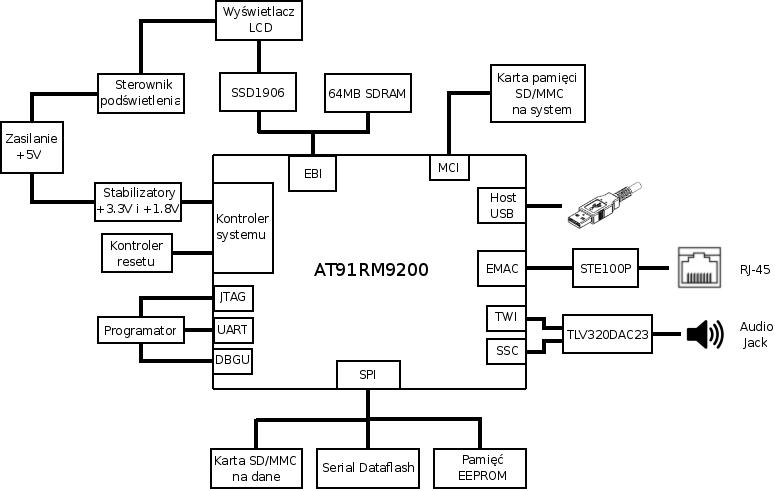
\includegraphics[scale=0.6]{img/schematic.jpg}
						\caption{Schemat blokowy projektu}
						\label{fig:block_schematic}
					\end{center}
				\end{figure}
				Rysunek \ref{fig:block_schematic} przedstawia schemat ideowy przykładowego rozwiązania platformy sprzętowej. Projekt zdecydowano wykonać w darmowej wersji programu do projektowania płytek drukowanych Eagle, jednak z powodu ograniczeń tej wersji (dozwolony maksymalny rozmiar pojedynczej płytki to 100mm*80mm) wystąpiła potrzeba podziału projektu na części opisane w punktach \ref{sec:main_board}, \ref{sec:ext_board} i \ref{sec:programator}. Podział taki spowodował uzyskanie projektu mniejszej wielkości oraz możliwość zmiany konfiguracji sprzętowej poprzez wymianę dodatkowej płytki PCB.\\
				Dwuwarstwowe płytki drukowane zostały wykonane w firmie Merkar z Katowic.\\
				Schematy ideowe, projekt PCB oraz zdjęcia wykonanego układu znajdują się w dodatku \ref{app:gotowy_projekt}.
			\subsection{Główna płytka sprzętowa}
				\label{sec:main_board}
				\subsubsection{Opis}
					Podstawowa część projektu jest w stanie samodzielnie obsługiwać system operacyjny Linux. W jej skład wchodzą:
					\begin{itemize}
						\item Mikroprocesor AT91RM9200
						\item Zasilanie układu oraz kontroler resetu
					\item 64MB pamięci SDRAM
						\item Złącze karty pamięci SD/MMC przeznaczonej na system operacyjny
						\item Sterownik warstwy fizycznej Ethernetu oraz gniazdko RJ-45
						\item Pamięć Serial Dataflash przechowująca programy uruchomieniowe
						\item Złącza dla programatora oraz dodatkowej płytki drukowanej
					\end{itemize}
					Za pomocą dwóch 40-pinowych złączy szpilkowych zostały wyprowadzone linie zasilania +3.3V i +5V oraz 54 linie ogólnego użytku, w tym magistrala EBI (External Bus Interface), TWI (Two Wire Interface), SPI (Serial Peripheral Interface), SSC (Synchronous Serial Controller).\\
				\subsubsection{Uwagi}
					\label{sec:uwagi}
					Podczas projektowania tej części platformy należało zwracać uwagę na wymienione poniżej zagadnienia.
					\begin{itemize}
						\item Do zasilania projektu użyto zasilacza impulsowego +5V/2.5A. Na wejściu zastosowano bezpiecznik 1.5A, diodę zabezpieczającą oraz serię kondensatorów elektrolitycznych i tantalowych.\\
						Ponieważ do działania układu jest dodatkowo konieczne napięcie +3.3V i +1.8V, zastosowano stabilizatory LM3940IMP-3.3 o maksymalnym obciążeniu prądowym 1A i LM1117-1.8 o obciążeniu 800mA.\\
						Napięcie +3.3V jest używane przez większość układów scalonych oraz transformator w gniazdku RJ-45. Do podświetlania wyświetlacza LCD jest potrzebne napięcie +5V, dlatego użyto bezpiecznika o dopuszczalnej wartości prądowej 1.5A.
						\item Ważne jest zapewnienie poprawnego startu mikrokontrolera dzięki podłączeniu pamięci Dataflash i zwarciu nóżki BMS mikrokontrolera poprzez opornik do napięcia zasilania. Po zresetowaniu mikrokontrolera zostanie uruchomiony program zawarty w pamięci ROM, który jest odpowiedzialny za przeszukanie kolejno pamięci Serial Dataflash podłączonej do portu SPI0, pamięci EEPROM dołączonej przez interfejs TWI oraz pamięci równoległej aktywowanej sygnałem NCS0, w celu znalezienia poprawnego wektora wskazującego na kod aplikacji. Jeśli taki wektor zostanie znaleziony to kod jest ładowany z danego układu do pamięci SRAM mikrokontrolera i stamtąd wykonywany. W przeciwnym razie nowy kod w postaci binarnej może zostać przesłany poprzez szeregowy interfejs DBGU za pomocą prokołu XModem lub łączem USB wykorzystując zaprojektowany przez Atmel protokół DFU (Device Firmware Upgrade). Po poprawnym ściągnięciu obrazu aplikacji do pamięci SRAM nastąpi wykonanie pierwszego rozkazu.\\
							W celu prawidłowego skonfigurowania portu szeregowego lub USB należy użyć rezonatora kwarcowego o jednej z wartości wskazanych w dokumentacji AT91RM9200 (np. 18.432MHz).
						\item Jako zewnętrzną pamięć SDRAM użyto dwóch kości o pojemności 32MB każda i szerokości słowa 16 bit. Aby uzyskać częstotliwość pracy magistrali powyżej 60MHz (przy takiej szybkości pracy linie używane do przesyłu danych zachowują się jak linie długie) należało zwracać szczególną uwagę na mogące wystąpić następujące problemy.
							\begin{itemize}
								\item Układy pamięci umieścić możliwie jak najbliżej procesora, aby skrócić czas propagacji sygnału. W projekcie udało się uzyskać minimalną długość linii ok. 20mm.
								\item Wszystkie ścieżki między procesorem a pamięcią powinny mieć jak najbardziej zbliżoną do siebie długość aby wyrównać czas propagacji sygnałów i impedancję linii. Z powodu braku miejsca na dwuwarstwowej płytce drukowanej wyrównanie długości nie było w pełni możliwe - uzyskano wartości rzędu 20-30mm.
							\end{itemize}
						\item Gniazda szpilkowe używane do połączenia z dodatkową płytką drukowaną powinny wyprowadzać jak najwięcej użytecznych linii sygnałowych oraz linie napięcia zasilania +3.3V i +5V.
					\end{itemize}
			\subsection{Dodatkowa płytka sprzętowa}
				\label{sec:ext_board}
				Na przykładowej dodatkowej płytce drukowanej znajdują się wymienione układy:
				\begin{itemize}
					\item Kontroler wyświetlacza LCD SSD1906, sterownik podświetlenia TPS61040 i złącza ZIF do podłączenia panelu TFT LQ043T3DX02.
					\item Przetwornik audio cyfrowo-analogowy TLV320DAC23 i gniazdo Jack 3.5mm dla słuchawek lub głośników aktywnych.
					\item Gniazdo na karty pamięci MicroSD do przechowywania danych użytkownika.
				\end{itemize}
				Podczas projektowania tej części platformy należało zwracać uwagę głównie na dostosowanie wymiarów w celu podłączenia do podstawowej płytki sprzętowej. Płytki są umieszczane jedna na drugiej i łączone za pomocą gniazda szpilkowego zatem żadne wystające elementy nie mogą znajdować się w tych samych rejonach. Dodatkowo istotne było właściwe ustawienie gniazda na taśmę wyświetlacza LCD.
			\subsection{Programator}
				\label{sec:programator}
				Aby zaoszczędzić miejsce na głównej płytce wchodzącej w skład projektu, zdecydowano że układy scalone, złącza, oraz pozostałe elementy używane tylko podczas programowania lub debuggowania układu będą znajdować się na osobnej płytce drukowanej dołączanej za pomocą 16-sygnałowego przewodu do transmisji danych. Programator zawiera zatem złącze do interfejsu JTAG, port szeregowy UART oraz port do debuggowania układu DBGU. Schemat ideowy programatora oraz projekt płytki drukowanej znajdują się na rysunku \ref{fig:programator} w dodatku \ref{app:gotowy_projekt}.
			\subsection{Lutowanie}
				Założeniem projektu było, aby był on możliwy do zlutowania bez potrzeby użycia zaawansowanego sprzętu. Do lutowania większości elementów wykorzystano zwykłą stację lutowniczą, jednak elementy o rozstawie nóżek 0.5mm (m.in. mikrokontroler AT91RM9200) przylutowano za pomocą stacji na gorące powietrze.
			
			\subsection{Problemy sprzętowe}
				W trakcie i po zlutowaniu projektu okazało się że wystąpiło kilka problemów:
				\begin{itemize}
					\item W projekcie płytki drukowanej zastosowano złe obudowy niektórych kondensatorów ceramicznych i rezonatora kwarcowego 32.768kHz.
					\item Po pierwszym uruchomieniu przepalił się bezpiecznik na wejściu układu. Po jego wymianie na bezpiecznik wielokrotny problem dalej występował - zauważono że jeden z kondensatorów tantalowych został wlutowany odwrotnie co powodowało duży pobór prądu przez układ.
					\item Podczas próby skomunikowania z układem poprzez JTAG okazało się że rozlutowane są nóżki procesora odpowiedzialne za przesył danych do programatora oraz źle przylutowany został przycisk resetujący układ przez co procesor był ciągle w stanie resetu. Po poprawieniu tych błędów komunikacja powiodła się.
					\item W projekcie programatora zastosowano zły schemat złącza DB-9 używanego do szeregowego przesyłu danych.
					\item Użyto złego schematu gniazda RJ-45 używanego przez port Ethernet co spowodowało niemożliwość używania sieci w projekcie.
					\item Ponieważ najpierw zaprojektowana i wykonana została podstawowa część platformy, podczas tworzenia dodatkowej płytki sprzętowej okazało się, że należy poprawić kilka elementów na głównej płytce PCB:
						\begin{itemize}
							\item Zapomniano o wyprowadzeniu napięcia zasilania +5V.
							\item Przydatny okazał się sygnał PCK0, który stanowi programowalny przez mikrokontroler sygnał zegarowy. Jest on używany przez układ SSD1906.
							\item W pierwotnej wersji projektu nie uwzględniono, że płytki znajdujące się w niedużej odległości jedna nad drugą, zawierają wystające elementy, takie jak kondensatory ceramiczne i złącza. Główna płytka sprzętowa została nieznacznie poprawiona pod tym względem.
						\end{itemize}
				\end{itemize}
				Wszystkie znalezione błędy zostały pomyślnie poprawione w ostatecznej wersji projektu.



%------------------------------------------------------------------------------------
% CZĘŚĆ PROGRAMOWA
%------------------------------------------------------------------------------------

	\chapter{Część programowa}
		\section{Wprowadzenie}
			Posiadając działającą platformę sprzętową można przejść do części programowej projektu, na którą składa się:
			\begin{itemize}
				\item Zapoznanie się ze sposobami programowej komunikacji, w tym samego programowania jak i debuggowania układu.
				\item Uruchomienie programu inicjalizującego (ang. bootloader), odpowiedzialnego za poprawne skonfigurowanie najważniejszych urządzeń sprzętowych zawartych w projekcie a następnie uruchomienie jądra systemu Linux.
				\item Konfiguracja i kompilacja linuksowego kernela.
				\item Utworzenie głównego systemu plików.
				\item Napisanie sterowników dla pozostałych potrzebnych urządzeń.
			\end{itemize}
			Dopiero na etapie programowania ujawnia się większość błędów sprzętowych zaistniałych w fazie projektowania platformy.
		\section{Programowanie układu}
		
			\subsection{OpenOCD}
				Aby połączyć się z układem mikroprocesorowym za pomocą złącza JTAG należy zastosować specjalne oprogramowanie, które pozwoli na przetworzenie poleceń użytkownika, wydawanych za pośrednictwem komputera PC, na odpowiednie polecenia protokołu JTAG.\\
				Jedną z takich aplikacji jest Open On-Chip Debugger\cite{website:openocd}, który działa na zasadzie serwera uruchamianego w tle i oczekującego na polecenia użytkownika.
				\subsubsection{Instalacja}
					Stabilną wersję OpenOCD można pobrać ze strony domowej projektu, jednak wersja 0.2.0 nie współdziałała poprawnie z zastosowanym w tej pracy układem sprzętowym JTAG. W związku z tym użyto działającej wersji numer 1679 dostępnej pod kontrolą źródeł SVN na stronie twórców.\\
					Aby skompilować i zainstalować aplikację należy doinstalować sterowniki odpowiednie dla obsługi sprzętowej używanego programatora JTAG. Na systemie operacyjnym Debian wystarczy, mając uprawnienia administratora, wydać komendę:\\
					\texttt{apt-get install libftdi1 libftdi-dev libusb-dev}\\
					W celu ściągnięcia i zainstalowania samej aplikacji należy wykonać ciąg następujących poleceń:\\
					\texttt{svn checkout -r 1679 svn://svn.berlios.de/openocd/trunk} - spowoduje pobranie z SVN-a odpowiedniej wersji OpenOCD\\
					\texttt{./bootstrap} - wstępna konfiguracja\\
					\texttt{./configure ----enable-maintainer-mode ----enable-ft2232\_libftdi ----prefix=/usr} - konfiguracja aplikacji; dołączenie biblioteki LibFTDI i ustawienie katalogu gdzie ma zostać zainstalowana na /usr\\
					\texttt{make \&\& make install} - kompilacja i instalacja\\
					Po poprawnym wykonaniu powyższych komend powinniśmy móc uruchomić oprogramowanie poprzez wykonanie polecenia \texttt{openocd}
					
				\subsubsection{Konfiguracja}
					Możliwe jest podanie opcji konfiguracyjnych bezpośrednio przy uruchomieniu OpenOCD lub zastosowanie plików konfiguracyjnych. Zgodnie z zaleceniami twórców, istotny jest podział konfiguracji na części istotne dla zastosowanego interfejsu służącego do programowania, używanego procesora oraz ustawień dodatkowych układów np. zewnętrznej pamięci SDRAM używanej w projekcie. W związku z tym ustawienia zostały podzielone na 4 części:
					\begin{itemize}
						\item{\texttt{openocd.cfg}}\\
							Główny plik konfiguracyjny definiujący m.in. używane porty.
							\begin{lstlisting}[basicstyle={\footnotesize\ttfamily}]
# Main configuration file
telnet_port 4444
gdb_port 3333
gdb_memory_map enable
gdb_flash_program enable
init
reset halt
							\end{lstlisting}
						\item{\texttt{interface/turtelizer.cfg}}\\
							Ustawienia interfejsu sprzętowego służącego do programowania.\\
							Opcja \texttt{jtag\_khz} służy do ustawiania szybkości interfejsu, lecz powinna być zmieniana dopiero po osiągnięciu odpowiedniej szybkości pracy mikroprocesora.
							\begin{lstlisting}[basicstyle={\footnotesize\ttfamily}]
# Configuration file for programming interface
interface ft2232
ft2232_device_desc "Turtelizer JTAG/RS232 Adapter"
ft2232_layout turtelizer2
ft2232_vid_pid 0x0403 0xbdc8			
jtag_khz 8
jtag_nsrst_delay 200
jtag_ntrst_delay 200
							\end{lstlisting}
						\item{\texttt{target/at91rm9200.cfg}}\\
							Opcje specyficzne dla zastosowanego mikroprocesora.
							\begin{lstlisting}[basicstyle={\footnotesize\ttfamily}]
# Configuration file for AT91RM9200 microprocessor
reset_config srst_only srst_pulls_trst

if { [info exists CHIPNAME] } {
   set  _CHIPNAME $CHIPNAME
} else {
   set  _CHIPNAME at91rm9200
}
if { [info exists ENDIAN] } {
   set  _ENDIAN $ENDIAN
} else {
   set  _ENDIAN little
}
if { [info exists CPUTAPID ] } {
   set _CPUTAPID $CPUTAPID
} else {
   set _CPUTAPID 0x05b0203f
}
# Never allow the following!
if { $_CPUTAPID == 0x15b0203f } {
   puts "-------------------------------------------------"
   puts "- ERR: TapID 0x15b0203f is wrong for at91rm9200 -"
   puts "- ERR: The board has a JTAG select jumper       -"
   puts "-------------------------------------------------"
}

jtag newtap $_CHIPNAME cpu -irlen 4 -ircapture 0x1 -irmask 0xf 
   -expected-id $_CPUTAPID

# Create the GDB Target.
set _TARGETNAME [format "%s.cpu" $_CHIPNAME]
target create $_TARGETNAME arm920t -endian $_ENDIAN -chain-position 
   $_TARGETNAME 
# AT91RM9200 has a 16K block of sram @ 0x0020.0000
$_TARGETNAME configure -work-area-virt 0x00200000 -work-area-phys 
   0x00200000 -work-area-size 0x4000 -work-area-backup 1
							\end{lstlisting}
						\item{\texttt{board/at91rm9200\_lab.cfg}}\\
							Dodatkowy plik który może zawierać komendy używane do ustawienia szybkości pracy mikroprocesora, konfiguracji odpowiednich układów wewnętrznych, pamięci SDRAM itp.
					\end{itemize}
				\subsubsection{Uruchamianie}
					W celu uruchomienia demona OpenOCD należy wywołać poniższą komendę, podając nazwy używanych plików konfiguracyjnych:\\
					\texttt{openocd -f openocd.cfg -f interface/turtelizer.cfg -f target/at91rm9200.cfg}\\
					Możliwe jest wtedy podłączenie się np. przez program telnet na odpowiedni port (\texttt{telnet localhost 4444}) i wykonanie przykładowych poleceń:
					\begin{itemize}
						\item\texttt{mdb <address>} - przeczytaj bajt spod podanego adresu
						\item\texttt{mwb <address> <value>} - zapisz bajt pod podany adres
						\item\texttt{reset} - resetuje mikroprocesor
						\item\texttt{halt} - zatrzymuje pracę mikroprocesora
						\item\texttt{resume} - wznawia pracę mikroprocesora
						\item\texttt{reg} - wyświetla lub ustawia zawartość rejestru, np. \texttt{reg pc 0} zeruje licznik rozkazów
						\item\texttt{bp <address> <length>} - ustawia breakpoint pod podanym adresem, <length> to długość rozkazu obsługiwana przez mikroprocesor
						\item\texttt{load\_image <file> <adress>} - załadowanie pliku binarnego pod wskazany adres
						\item\texttt{arm920t cache\_info} - informacja o pamięci Cache zastosowanej w rdzeniu ARM920T
						\item\texttt{help} - pełny spis poleceń
					\end{itemize}
				
			\subsection{Debug Unit (DBGU)}
				Debug Unit jest sprzętowym interfejsem mikrokontrolera, który pozwala na szeregowe przesyłanie danych pomiędzy programowanym układem a komputerem PC. Za pomocą jednostki DBGU można w całości zaprogramować platformę, bez potrzeby stosowania interfejsu JTAG.\\
				Aby komputer klasy PC mógł się poprawnie komunikować z mikrokontrolerem należy użyć szeregowego kabla typu null-modem oraz programu takiego jak HyperTerminal (Windows) lub minicom (Linux) i zastosować następujące parametry transmisji:\\
				\texttt{szybkość transmisji: 115200,\\ilość bitów danych: 8,\\bit parzystości:brak,\\bity stopu: 1}\\
				Po uruchomieniu platformy, na ekranie terminala (np. minicom) powinien pojawiać się znak 'C' zachęcający do rozpoczęcia transmisji danych. Niezaprogramowany mikrokontroler oczekuje w ten sposób na przesłanie kodu programu poprzez protokół XModem. Po otrzymaniu kodu binarnego zostaje on skopiowany do wewnętrznej pamięci SRAM, a następnie stamtąd uruchomiony.\\
				Bardziej szczegółowy opis postępowania podczas programowania znajduje się w sekcji \ref{sec:bootloader2nd}.
			\subsection{Środowisko do kompilowania}
				W celu skompilowania kodu źródłowego dla procesora o architekturze ARM należy użyć kompilatora skrośnego (ang. cross compiler). Kompilator taki jest uruchamiany na standardowym komputerze PC, ale zamiast kompilować kod do rozkazów np. procesora x86, potrafi kompilować i optymalizować programy dla architektury ARM. Oczywiście posiadając działający system oparty o mikroprocesor z rodziny ARM, można na nim zainstalować natywny kompilator i przeprowadzać kompilację do właściwej postaci, jednak zazwyczaj, z uwagi na dużą częstotliwość pracy najnowszych procesorów w zwykłych komputerach PC, szybciej i prościej jest przeprowadzić kompilację z użyciem kompilatora skrośnego.\\
				Podczas wyboru odpowiedniego kompilatora, nie zawsze najlepszym wyjściem jest pobranie najnowszych dostępnych wersji - należy zwrócić uwagę na kompatybilność kompilatora z dodatkowymi bibliotekami i aplikacjami takimi jak np. linker ld i debugger gdb. Kompilator używany do kompilacji programów dla innej architektury można zbudować samemu, jednak najlepiej zastosować stabilne i przetestowane środowisko (tzw. toolchain), które zostało już skompilowane dla danej architektury i posiada spełnione wszystkie wymagane zależności.\\
				W projekcie zastosowano toolchain pobrany ze strony \cite{website:gnuarm}, w którego skład wchodzi kompilator gcc-4.0.2-c-c++, dodatkowe aplikacje binarne binutils-2.16.1, oraz biblioteka C przeznaczona dla systemów wbudowanych newlib-1.14.0.

			\subsection{Eclipse}
				Podczas pisania oprogramowania, warto jest zastosować efektywne środowisko programistyczne, które może znacznie ułatwić proces tworzenia części programowej projektu.\\
				Jedną z popularniejszych aplikacji tego typu jest środowisko Eclipse, które pozwala na pisanie i kompilowanie oprogramowania w języku C, a także po odpowiedniej konfiguracji jego testowanie i debuggowanie na docelowej platformie dzięki zastosowaniu interfejsu JTAG. Szczegółowy opis konfiguracji został przedstawiony na stronie projektu YAGARTO\cite{website:yagarto}.
				
		\section{Bootloader}
			Bootloader, czyli pierwszy program uruchamiany po zresetowaniu mikrokontrolera, jest odpowiedzialny za zainicjalizowanie podstawowej funkcjonalności platformy, a następnie uruchomienie jądra systemu Linux. Mikrokontroler AT91RM9200 posiada wbudowany program inicjalizujący pierwszego poziomu, którego działanie zostało opisane w sekcji \ref{sec:uwagi}.\\
			Ponieważ program załadowany z Serial Dataflasha do pamięci SRAM może zajmować co najwyżej 16kB (w tym oprócz samego kodu należy uwzględnić obszar pamięci potrzebny na dane użytkownika) jego funkcjonalność jest znacznie ograniczona. Bardzo trudnym lub niewykonalnym zadaniem jest aby w tak niewielkiej ilości pamięci zmieścić aplikację, która będzie odpowiedzialna za skonfigurowanie pamięci SDRAM, odczytanie kernela z karty pamięci lub sieci i uruchomienie go. Dlatego zdecydowano się że program zawarty w pamięci ROM pobierze z pamięci Serial Dataflash i uruchomi bootloader drugiego poziomu (nazwany LAB Bootloader), którego zadaniem będzie konfiguracja pamięci SDRAM i wczytanie do niej głównego programu inicjalizującego. Dopiero główny bootloader, posiadający znacznie bardziej zaawansowaną funkcjonalność, zajmie się uruchomieniem jądra systemu operacyjnego Linux.\\
			Obydwa programy inicjalizujące są zapisane w pamięci Serial Dataflash (w projekcie użyto układu AT45DB041D o pojemności 512kB), ich rozmieszczenie zostało przedstawione na rysunku \ref{fig:bootloader_map}.
			\begin{figure}[]
				\begin{center}
					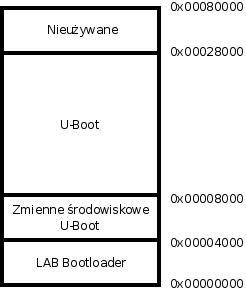
\includegraphics[scale=0.6]{img/bootloader_map.jpg}
					\caption{Zawartość pamięci Serial Dataflash}
					\label{fig:bootloader_map}
				\end{center}
			\end{figure}
			\subsection{Bootloader inicjalizujący}
				\label{sec:bootloader2nd}
				Jako bootloader drugiego poziomu (LAB Bootloader), czyli pierwszą aplikację której kod źródłowy jest dostępny dla użytkownika, zdecydowano się użyć stworzony przez firmę Atmel projekt RomBoot dla zestawu AT91RM9200DK\cite{website:arm_booting}. Kod został przeportowany dla kompilatora gcc zamiast ADS (ARM Developer Suite) a następnie nieznacznie uproszczony i dostosowany do potrzeb platformy sprzętowej. Zadaniem tego programu jest wykonanie następujących operacji:
				\begin{enumerate}
					\item Inicjalizacja wektorów przerwań i konfiguracja stosów dla różnych trybów pracy mikrokontrolera.
					\item Inicjalizacja kontrolera przerwań.
					\item Ustawienie poprawnej szybkości pracy procesora.
					\item Skonfigurowanie pamięci synchronicznej SDRAM.
					\item Zapoczątkowanie komunikacji poprzez port do debuggowania układu DBGU.
					\item Wyczyszczenie pamięci cache, ustawienie poprawnego trybu pracy układu, zezwolenie na przerwania.
					\item Inicjalizacja pamięci Serial Dataflash.
				\end{enumerate}
				Po pomyślnym wykonaniu powyższych czynności mikrokontroler automatycznie wystartuje główny program inicjalizujący po upływie określonego czasu (domyślnie 0.5 sekundy) lub będzie czekał na polecenia użytkownika. Obecna wersja aplikacji umożliwia wykonanie następujących poleceń:
				\begin{itemize}
					\item Pobranie danych poprzez port szeregowy pod wskazany adres pamięci Serial Dataflash.
					\item Przeczytanie zawartości pamięci SDRAM pod podanym adresem.
					\item Przeczytanie zawartości pamięci Serial Dataflash pod podanym adresem.
					\item Wystartowanie głównego bootloadera.
					\item Wyczyszczenie obszaru pamięci Dataflash zajmowanego przez podstawowy program inicjalizujący.
					\item Informacja o pamięci i bootloaderze.
				\end{itemize}
				Skompilowany i zoptymalizowany kod tego bootloadera zajmuje ok. 11kB. Rozmiar ten można jeszcze zmniejszyć ponieważ mikrokontroler AT91RM9200 umożliwia poprzez tzw. Embedded Software Services wykorzystanie funkcji które znajdują się w pamięci ROM i są używane przez bootloader pierwszego poziomu.
				
			\subsection{Bootloader główny}
				Po analizie dostępnych rozwiązań, zdecydowano że jako główny bootloader zostanie użyty projekt U-Boot autorstwa Wolfganga Denka\cite{website:uboot}. Wybrany projekt został w znacznej mierze oparty na źródłach systemu operacyjnego Linux oraz posiada wsparcie dla mikrokontrolera AT91RM9200.\\
				Po pobraniu z internetu i poprawnym skompilowaniu za pomocą polecenia \texttt{make} przystąpiono do dostosowywania aplikacji do potrzeb docelowej platformy sprzętowej. W tym celu do katalogu \texttt{board/atmel/lab\_at91rm9200} skopiowano zawartość przykładowego projektu zawartego w \texttt{board/atmel/at91rm9200dk} i w dalszej kolejności wykonano następujące czynności:
				\begin{enumerate}
					\item Zmodyfikowano nazwę głównego pliku \texttt{at91rm9200dk.c} na \texttt{lab\_at91rm9200.c} i wszystkie nazwy oraz ścieżki w pliku \texttt{Makefile}.
					\item W pliku źródłowym \texttt{lab\_at91rm9200.c} usunięto funkcje odpowiedzialne za konfigurację pamięci NAND oraz zmieniono funkcję inicjalizującą interfejs sieciowy.
					\item W pliku \texttt{partition.c} zmieniono konfigurację zawartości pamięci Serial Dataflash (p. rys. \ref{fig:bootloader_map}).
					\item Do katalogu \texttt{cpu/arm920t/at91rm9200/}, który zawiera pliki źródłowe specyficzne dla zastosowanego mikrokontrolera skopiowano brakujące pliki:
						\begin{itemize}
							\item \texttt{atmel\_mci.c} - funkcje do obsługi interfejsu MCI
							\item \texttt{atmel\_mci.h} - plik nagłówkowy używany przez funkcje obsługujące MCI
							\item \texttt{ste100p.c} - funkcje do obsługi warstwy fizycznej interfejsu sieciowego
							\item \texttt{ste100p.h} - plik nagłówkowy używany przez powyższy plik źródłowy
						\end{itemize}
					\item W pliku \texttt{Makefile} w katalogu \texttt{cpu/arm920t/at91rm9200/} dodano wpisy dla plików obiektowych \texttt{atmel\_mci.o} i \texttt{ste100p.o}.
					\item Zmieniono pliki \texttt{drivers/mtd/dataflash.c} i \texttt{include/dataflash.h} pod kątem zastosowanego układu pamięci Serial Dataflash AT45DB041D.
					\item Dodano plik \texttt{include/asm-arm/arch-at91rm9200/mmc.h}.
					\item W pliku \texttt{include/configs/lab\_at91rm9200.h} utworzonym na podstawie przykładowego pliku konfiguracyjnego zmodyfikowano wartości takie jak szybkość pracy mikroprocesora, ilość dostępnej pamięci SDRAM oraz opcje dostępne w menu U-Boot.
					\item Dodano wpis dla platformy \texttt{lab\_at91rm9200} w głównym pliku \texttt{Makefile} projektu U-Boot oraz zmieniono ścieżkę dostępu do używanego kompilatora.
				\end{enumerate}
				Skompilowany kod w postaci binarnej umieszczono pod adresem 0x00008000 w pamięci Serial Dataflash za pomocą opcji dostępnej w bootloaderze inicjalizującym.\\
				\subsubsection{Uruchamianie}
				Pierwsze próby uruchomienia nie powiodły się - po zdebuggowania z użyciem JTAG-u okazało się że procesor wykonuje skok pod zły adres w pamięci. Ponieważ U-Boot jest uruchamiany z poziomu pamięci SDRAM sugerowało to problemy z czasami dostępu. Zewnętrzna magistrala używana podczas dostępu do pamięci była taktowana zegarem o częstotliwości 60MHz, niestety obniżenie szybkości pracy nie poprawiło efektów działania procesora.\\
				W pewnym stopniu pomogło wyłączenie w procesorze pamięci cache dla instrukcji. Spowodowało to jednak kilkukrotne spowolnienie działania układu, ponieważ kolejne rozkazy dla procesora były za każdym razem pobierane z pamięci SDRAM.\\
				W dalszej kolejności postanowiono sprawdzić poprawność działania pamięci SDRAM podczas szybkiego czytania i zapisywania danych. Aby tego dokonać napisano prostą aplikację opartą o bootloader inicjalizujący, której zadaniem było przeprowadzenie szeregu testów opisanych w dalszej części pracy.
				\begin{itemize}
 					\item \textbf{test adresowy} - Ten test zapisuje unikalną wartość w każdej komórce pamięci. Przykładowo moży to być adres tej komórki. Po zapisaniu dane są odczytywane i sprawdzane. 
					\item \textbf{maszerujący wzorzec} - Algorytm czyści zawartość pamięci, następnie odczytuje zawartość pierwszej komórki i zapisuje do niej wartość 1. Ta procedura odczytu i zapisu jest powtarzana dla wszystkich lokacji w pamięci. W tym momencie cała pamięć powinna być zapełniona liczbami 1. Kolejnym etapem testu jest poruszanie się od końca pamięci, odczyt kolejnych komórek i zamiana ich zawartości na 0. Po osiągnięciu początku pamięci test jest powtarzany z użyciem dopełnionych wartości.
					\item \textbf{galopujący wzorzec} - Test sprawdzający niepowtarzalność adresów i inne funkcjonalne błędy w pamięci, jak również niektóre dynamiczne przekłamania. Algorytm odwołuje się do każdej komórki pamięci używając po kolei każdego z pozostałych adresów jako miejsca, z którego nastąpi skok do sprawdzanej lokacji. Po wyczyszczeniu pamięci pierwsza komórka staje się adresem testowym - jest ona dopełniana i sprawdzana na zmianę z każdym z pozostałych adresów w całej pamięci. Każda kolejna komórka przyjmuje rolę testowej aż do momentu sprawdzenia całości.\\
					Z powodu dużej złożoności czasowej tego algorytmu, sprawdzono tylko kilka obszarów wielkości 1kB (czas wykonania takiego testu to ok. 40 minut).
				\end{itemize}
				Przeprowadzenie powyższych testów dla słów o długości 1, 2 i 4 bajtów nie wykazało żadnych błędów.\\
				Jak się okazało, problem stanowiła zbyt duża różnica w czasie dostępu do wbudowanej pamięci cache a zewnętrznej pamięci SDRAM. Rdzeń procesora taktowany zegarem 180MHz działał zbyt szybko podczas próby pobrania rozkazu z zewnętrznej pamięci, która korzystała z zegara o częstotliwości 60MHz. Po podwyższeniu tej wartości do 90MHz uruchomienie bootloadera U-Boot powiodło się.
		\section{Linux}
			W tym rozdziale zostanie opisany przebieg instalacji systemu operacyjnego Linux na docelowej platformie sprzętowej. Linux jest bardzo rozbudowanym systemem i daje użytkownikowi wiele możliwości konfiguracji, zarówno na etapie kompilacji jądra, jak i po uruchomieniu. Ponieważ celem tej pracy jest uruchomienie wbudowanej wersji Linuksa, na tym etapie należy zwrócić szczególną uwagę na wybór modułów wspieranych przez jądro, używaną dystrybucję (zestaw podstawowych aplikacji) oraz system plików.
			\subsection{Jądro systemu}
				\label{sec:linux_kernel}
				Jądro Linuksa jest w dużym stopniu zgodne ze standardami ANSI i POSIX, obsługuje wielozadaniowość, wielowątkowość, wielobieżność, pamięć wirtualną, biblioteki współdzielone, ładowanie na żądanie, współdzielony kod wykonywalny (ang. copy-on-write), dobre zarządzanie pamięcią i obsługę sieci TCP/IP.\\
				Poprzez zastosowanie modułowej budowy, można w trakcie konfiguracji zdecydować czy system powinien wspierać wybrane urządzenia, protokoły i inne funkcjonalności. Dzięki temu można dostosować kernel do konkretnych zadań, zmniejszyć ilość zajmowanej przez niego pamięci operacyjnej oraz zoptymalizować jego działanie.
				\subsubsection{Konfiguracja}
					W projekcie zdecydowano wykorzystać jądro systemu operacyjnego Linux w wersji 2.6.27.8 - jest to stabilne wydanie kernela, które zostało użyte w jednym z przykładowych projektów zawartych w dodatku \ref{app:przykladowe_projekty}, zatem posiadano pewność że ta wersja powinna działać.\\
					Spakowane archiwum zawierające źródła systemu operacyjnego należy pobrać ze strony internetowej \url{http://kernel.org/}, natomiast przydatne jest dodatkowo pobranie ze strony \url{http://maxim.org.za/at91_26.html} pliku z drobnymi poprawkami dla mikrokontrolera AT91RM9200 (plik jest dostępny w dołączonych materiałach). Aby go zastosować należy w głównym katalogu ze źródłami Linuksa wykonać polecenie:\\
					\texttt{patch -p0 < 2.6.27-at91.patch.gz}\\
					W dalszej kolejności należało wprowadzić modyfikacje niezbędne dla zastosowanej platformy sprzętowej m.in.
					\begin{itemize}
						\item Dodanie pliku \texttt{arch/arm/mach-at91/board-lab-at91rm9200.c} zawierającego funkcje używane podczas inicjalizacji płytki sprzętowej.
						\item Dołączenie w plikach \texttt{arch/arm/mach-at91/Kconfig} i \texttt{arch/arm/mach-at91/Makefile} nowych obiektów potrzebnych podczas konfiguracji i kompilacji.
						\item Dodanie obsługi warstwy fizycznej dla interfejsu sieciowego STE100P.
					\end{itemize}
					Powyższe poprawki są uwzględnione w pliku \texttt{linux-2.6.27.8-lab\_at91rm9200.patch.gz}.\\
					Po zastosowaniu wszystkich poprawek można przystąpić do wyboru konkretnych opcji konfiguracyjnych kernela - aby w tym celu skorzystać z pomocy graficznego narzędzia, należy wykonać polecenie \texttt{make ARCH=arm xconfig}.\\
					Uruchomiona w ten sposób aplikacja, zależnie od wybranej architektury sprzętowej procesora, dzieli strukturę kernela na kilkanaście kategorii. Ich opis wraz z objaśnieniem wyboru modułów został przedstawiony poniżej.
				\subsubsection{Kompilacja}
					k
			\subsection{Dystrybucja}
				f
				\subsubsection{Buildroot}
					b
			\subsection{System plików}
				s
			\subsection{Uruchamianie}
				u
				% jak u-boot to startuje? wylaczone przerwania, d-cache i i-cache
			\subsection{Dodatkowe moduły}
				\label{sec:linux_modules}
				m
				\subsubsection{Ethernet}
				\subsubsection{Kontroler LCD}
%		\section{Aplikacja demonstracyjna}
		
	\chapter{Podsumowanie}

	\bibliographystyle{plain}
	\bibliography{bibliography}
	
	
	
	\appendix
	
	\chapter{Gotowy projekt}
	\label{app:gotowy_projekt}
%		\begin{figure}[h]
%			\begin{center}
%				\label{fig:cpu_sch}
%				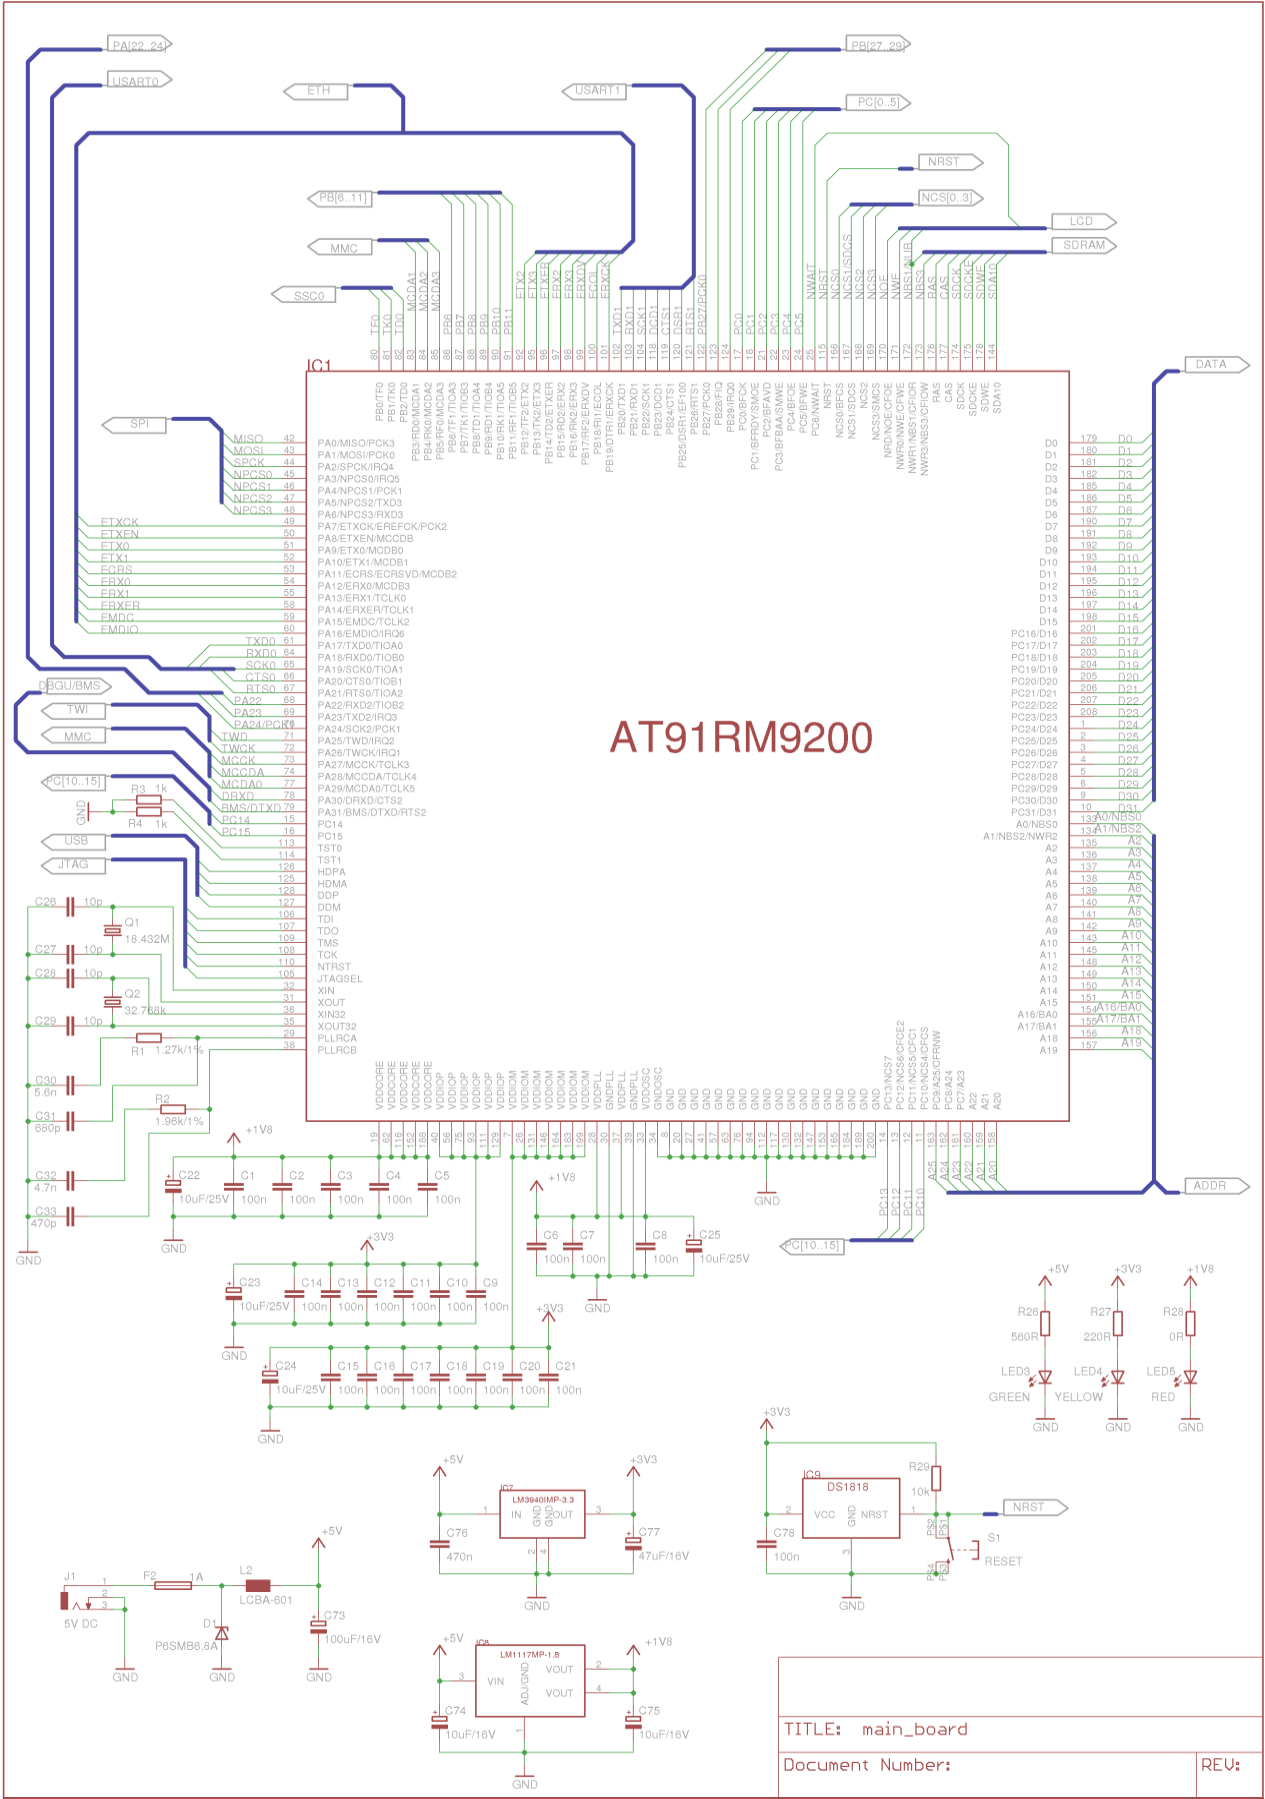
\includegraphics[scale=1.0]{img/cpu_sch.png}
%				\caption{Schemat podłączenia mikrokontrolera}
%			\end{center}
%		\end{figure}
%		
%		\begin{figure}[h]
%			\begin{center}
%				\label{fig:main_sch}
%				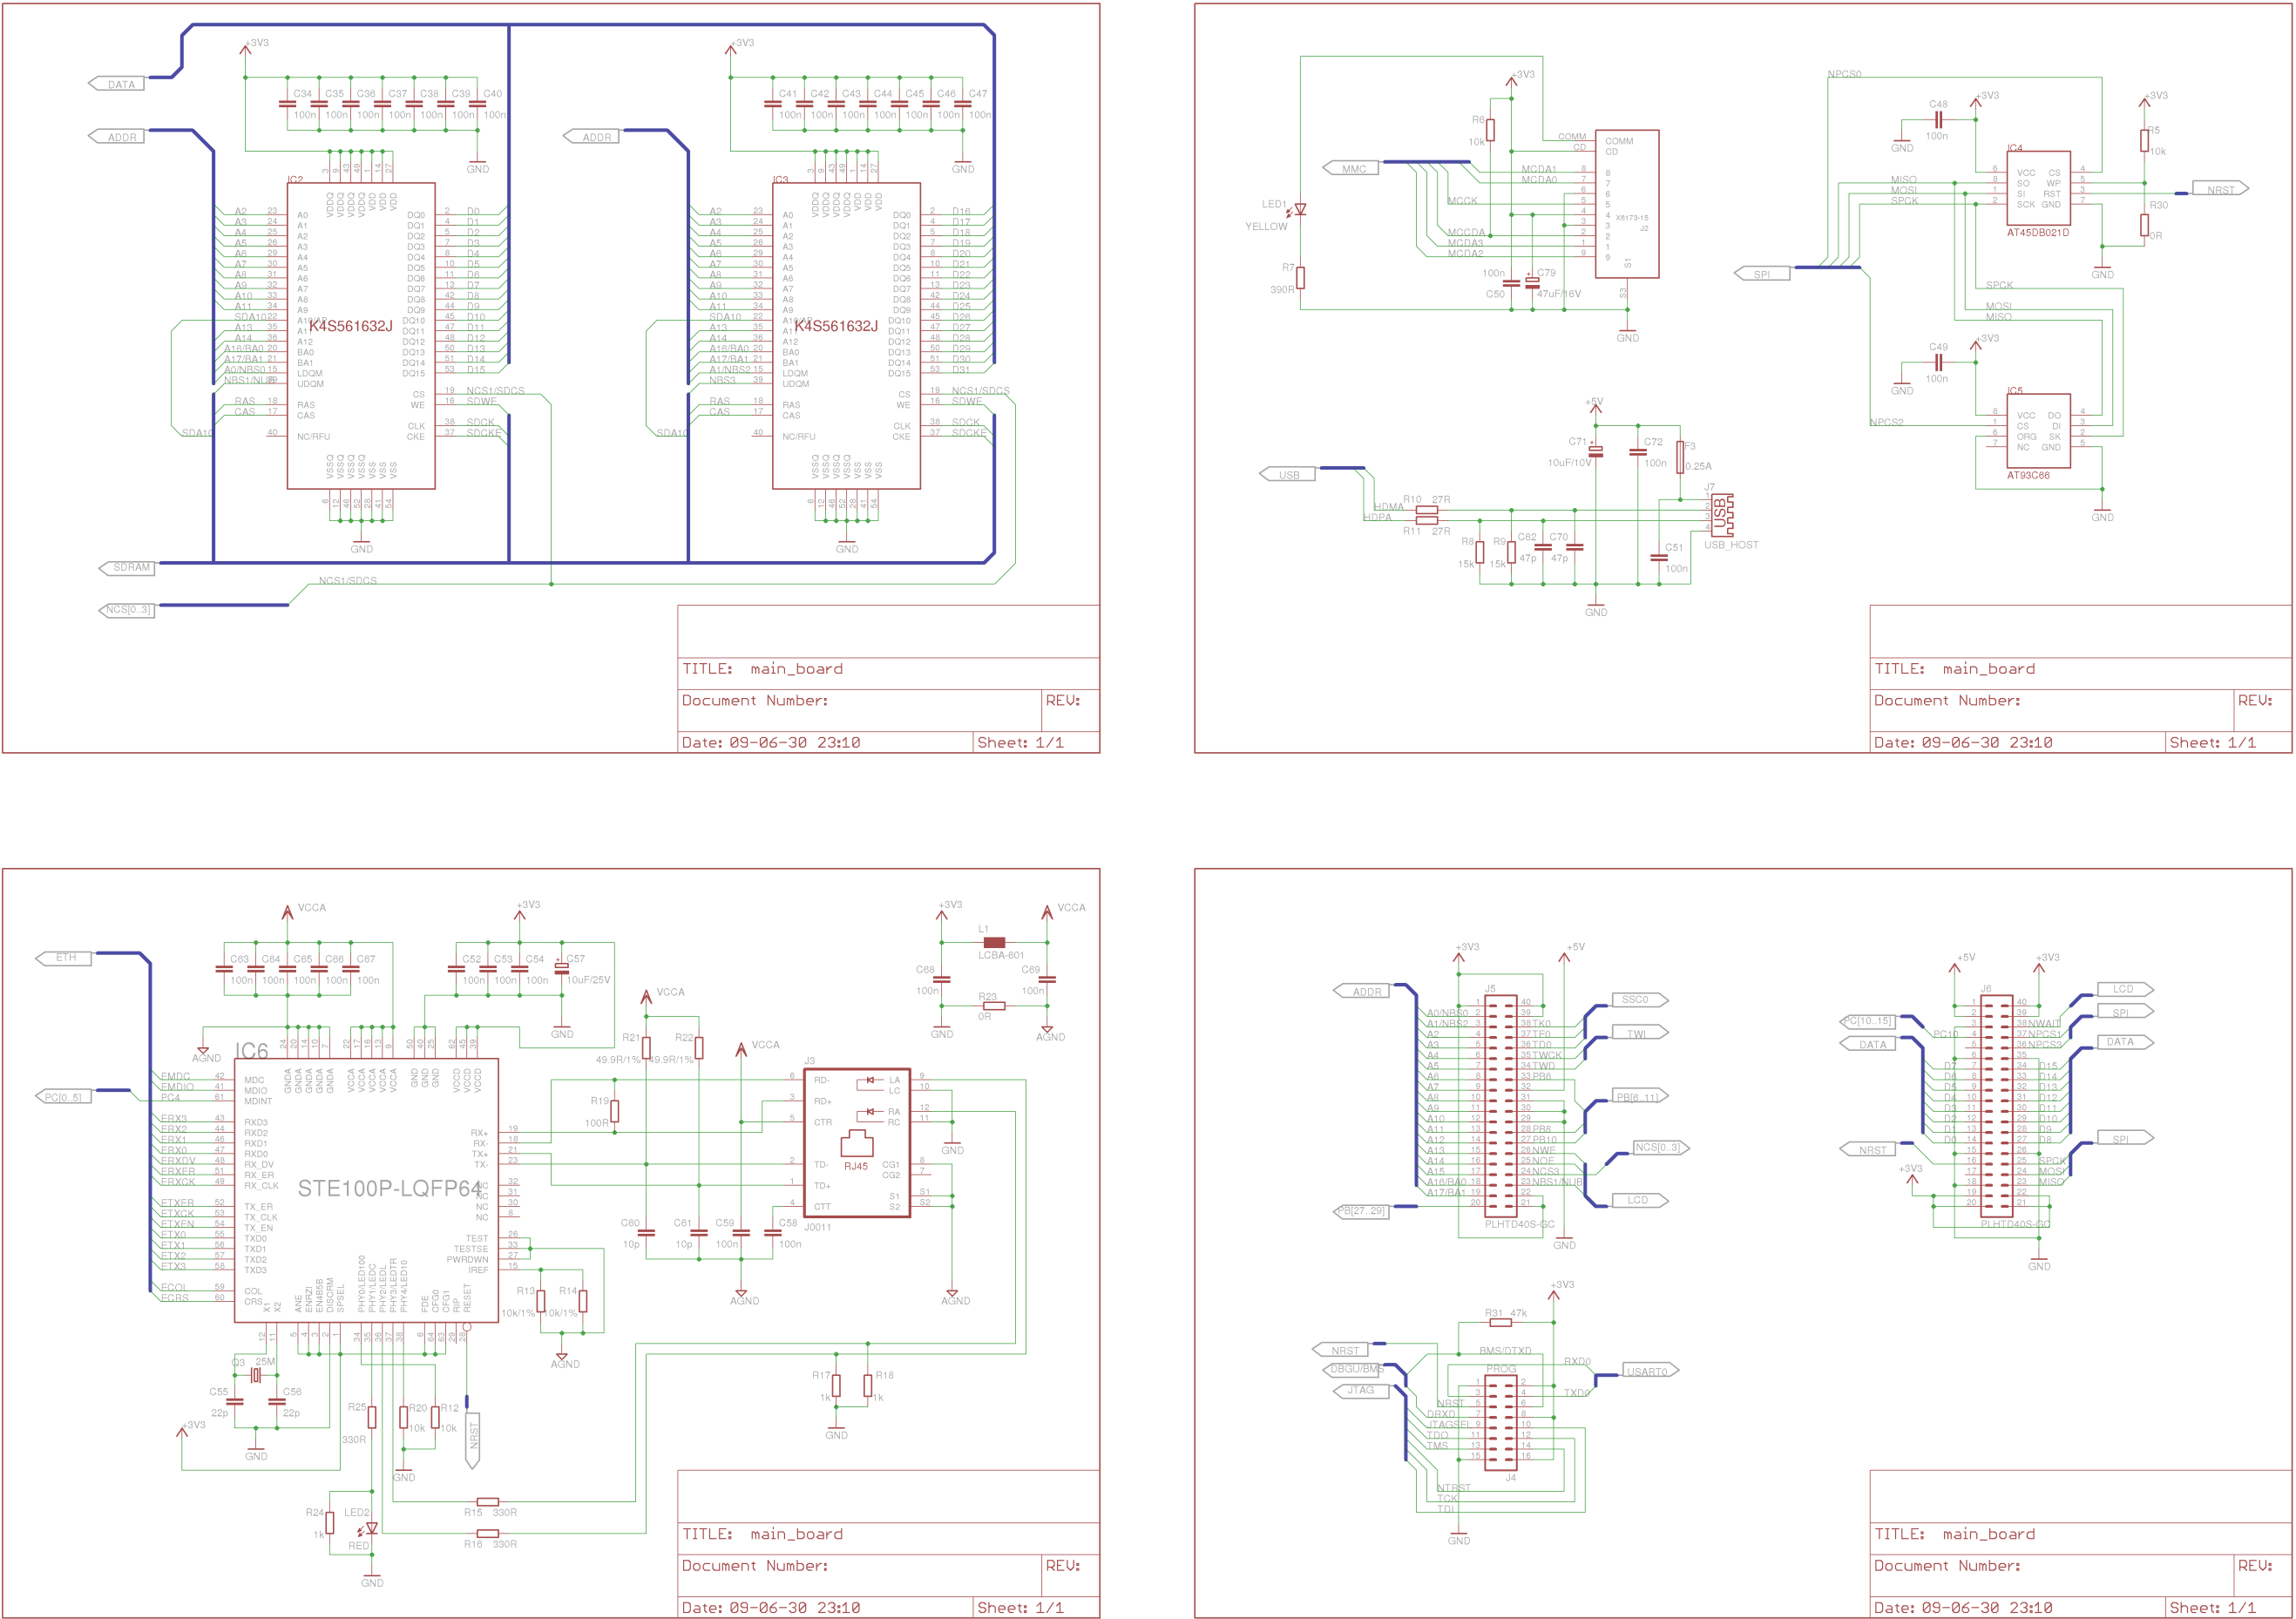
\includegraphics[scale=1.0,angle=90]{img/main_sch.png}
%				\caption{Schemat podłączenia dodatkowych układów do głównej części projektu}
%			\end{center}
%		\end{figure}
%		
%		\begin{figure}[h]
%			\begin{center}
%				\label{fig:ext_sch_lcd}
%				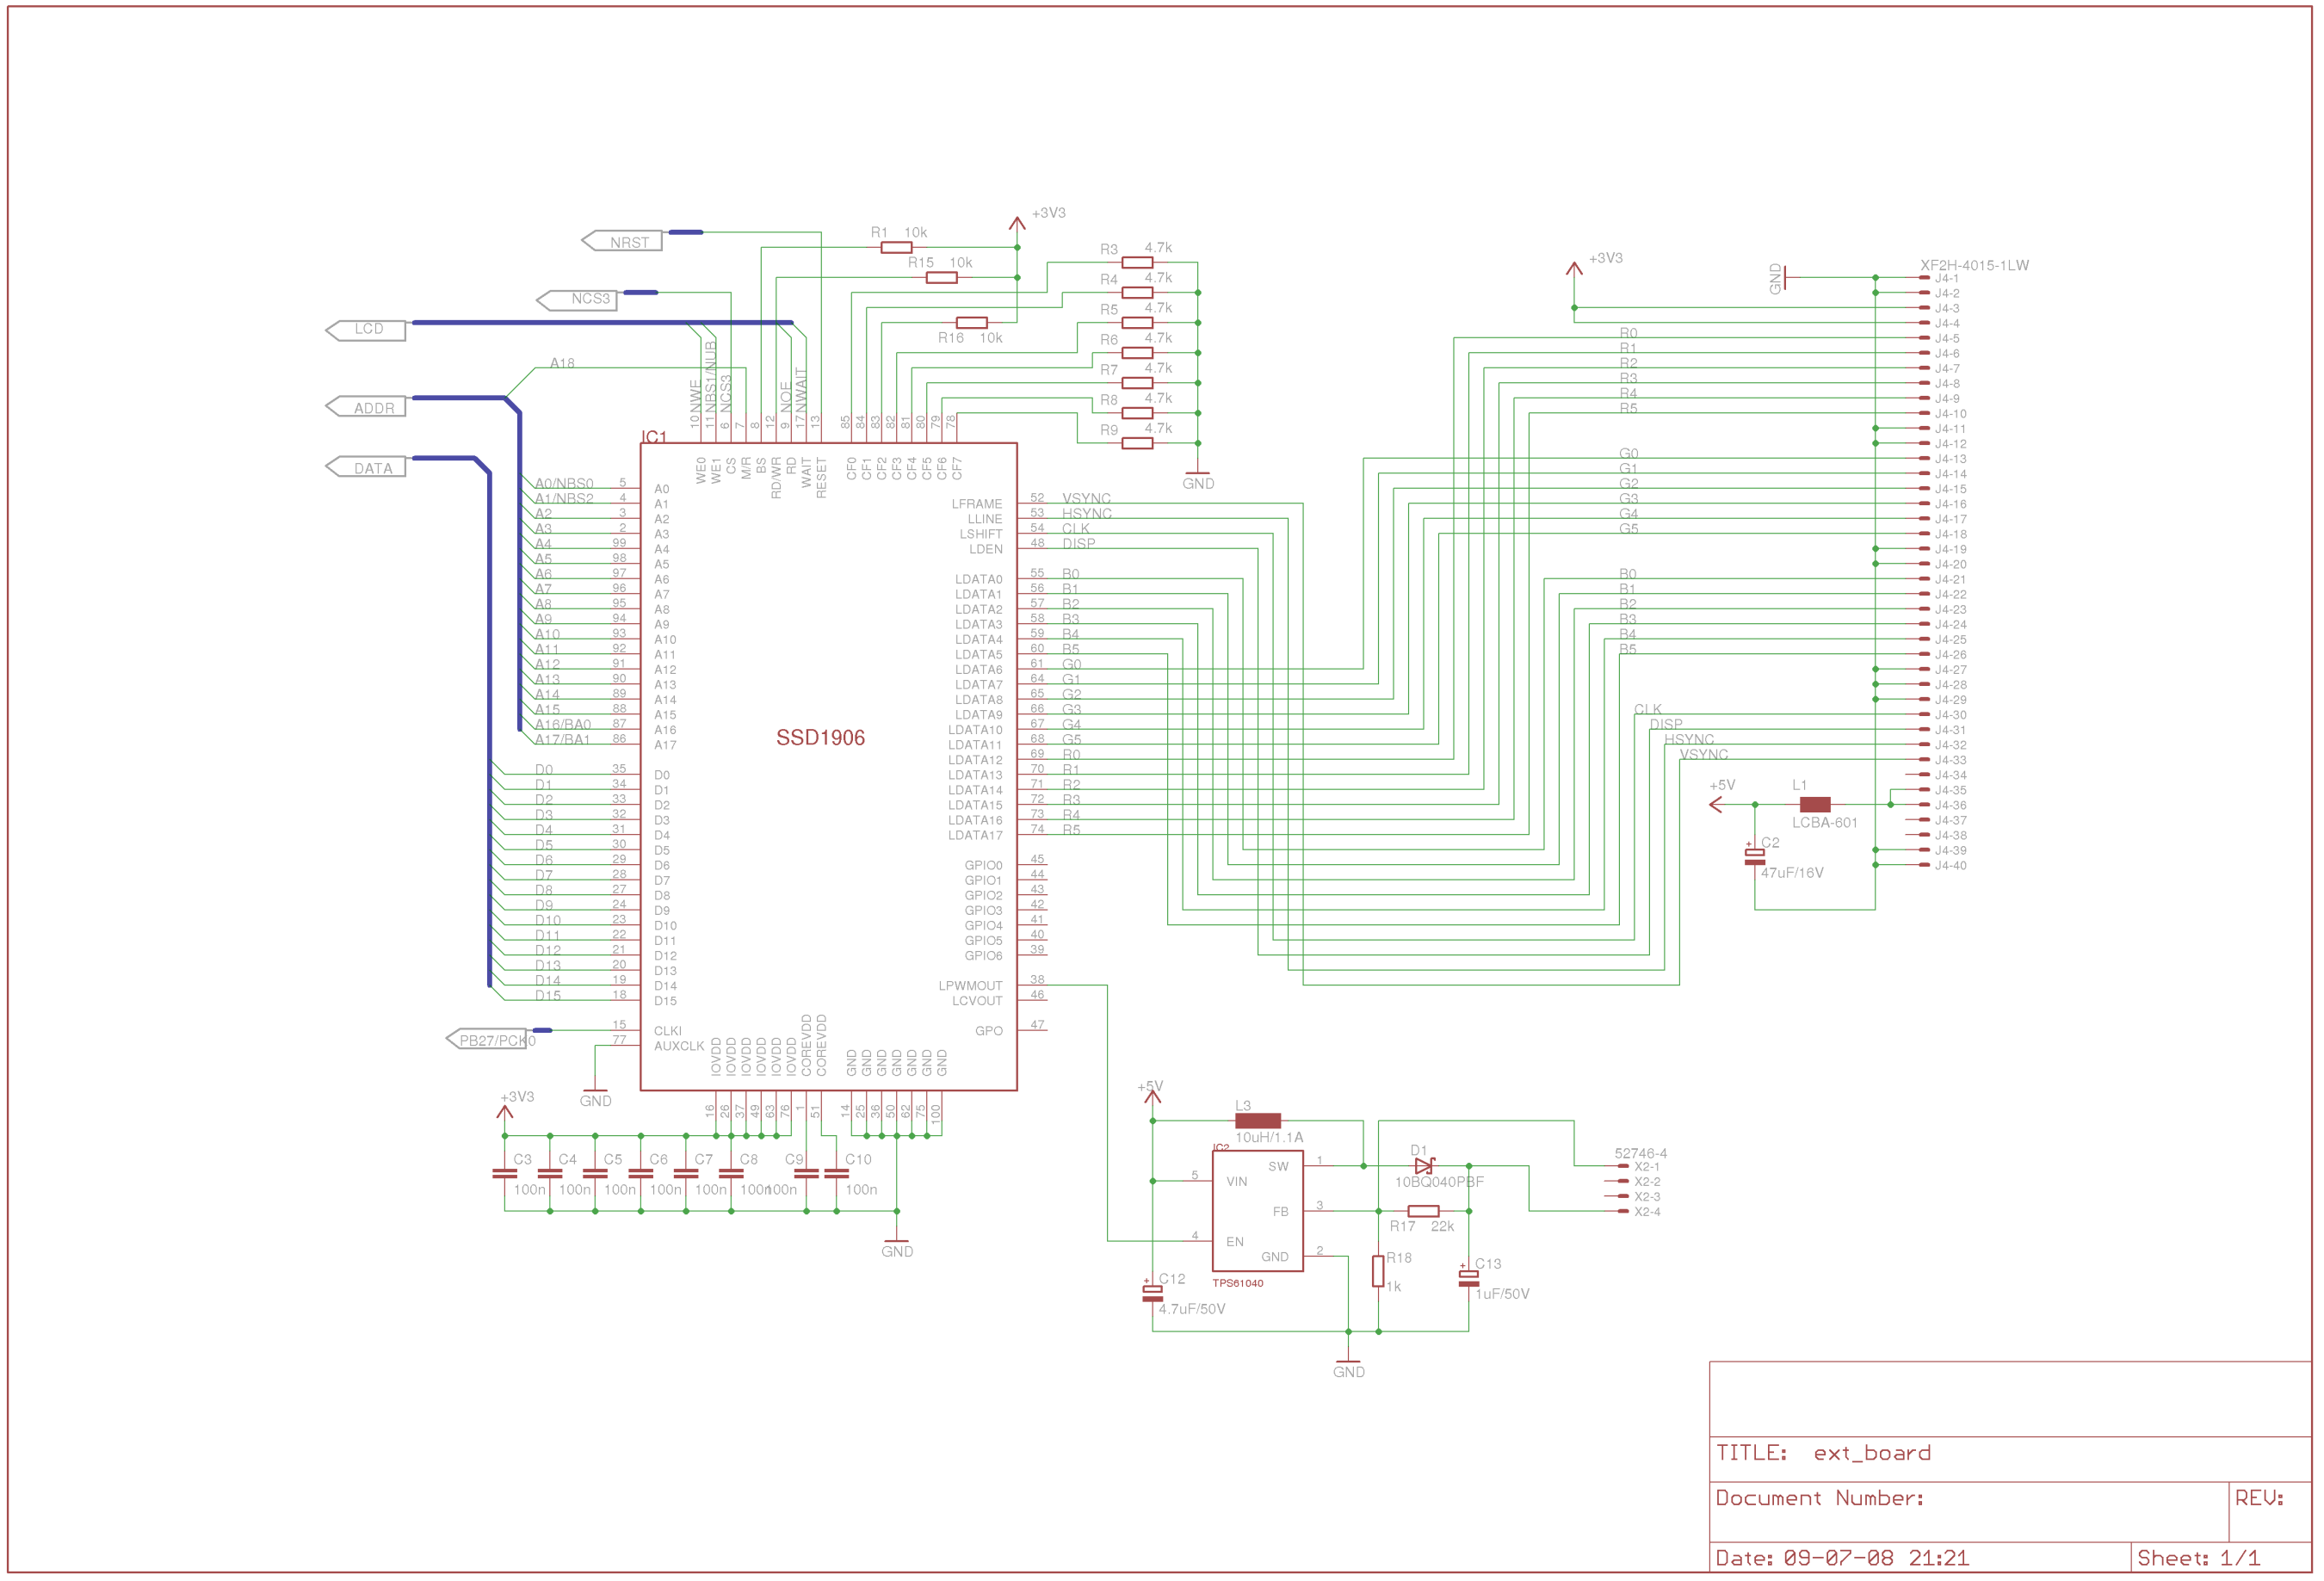
\includegraphics[scale=1.0,angle=90]{img/ext_sch1.png}
%				\caption{Schemat podłączenia wyświetlacza i kontrolera LCD}
%			\end{center}
%		\end{figure}
%		
%		\begin{figure}[h]
%			\begin{center}
%				\label{fig:ext_sch_rest}
%				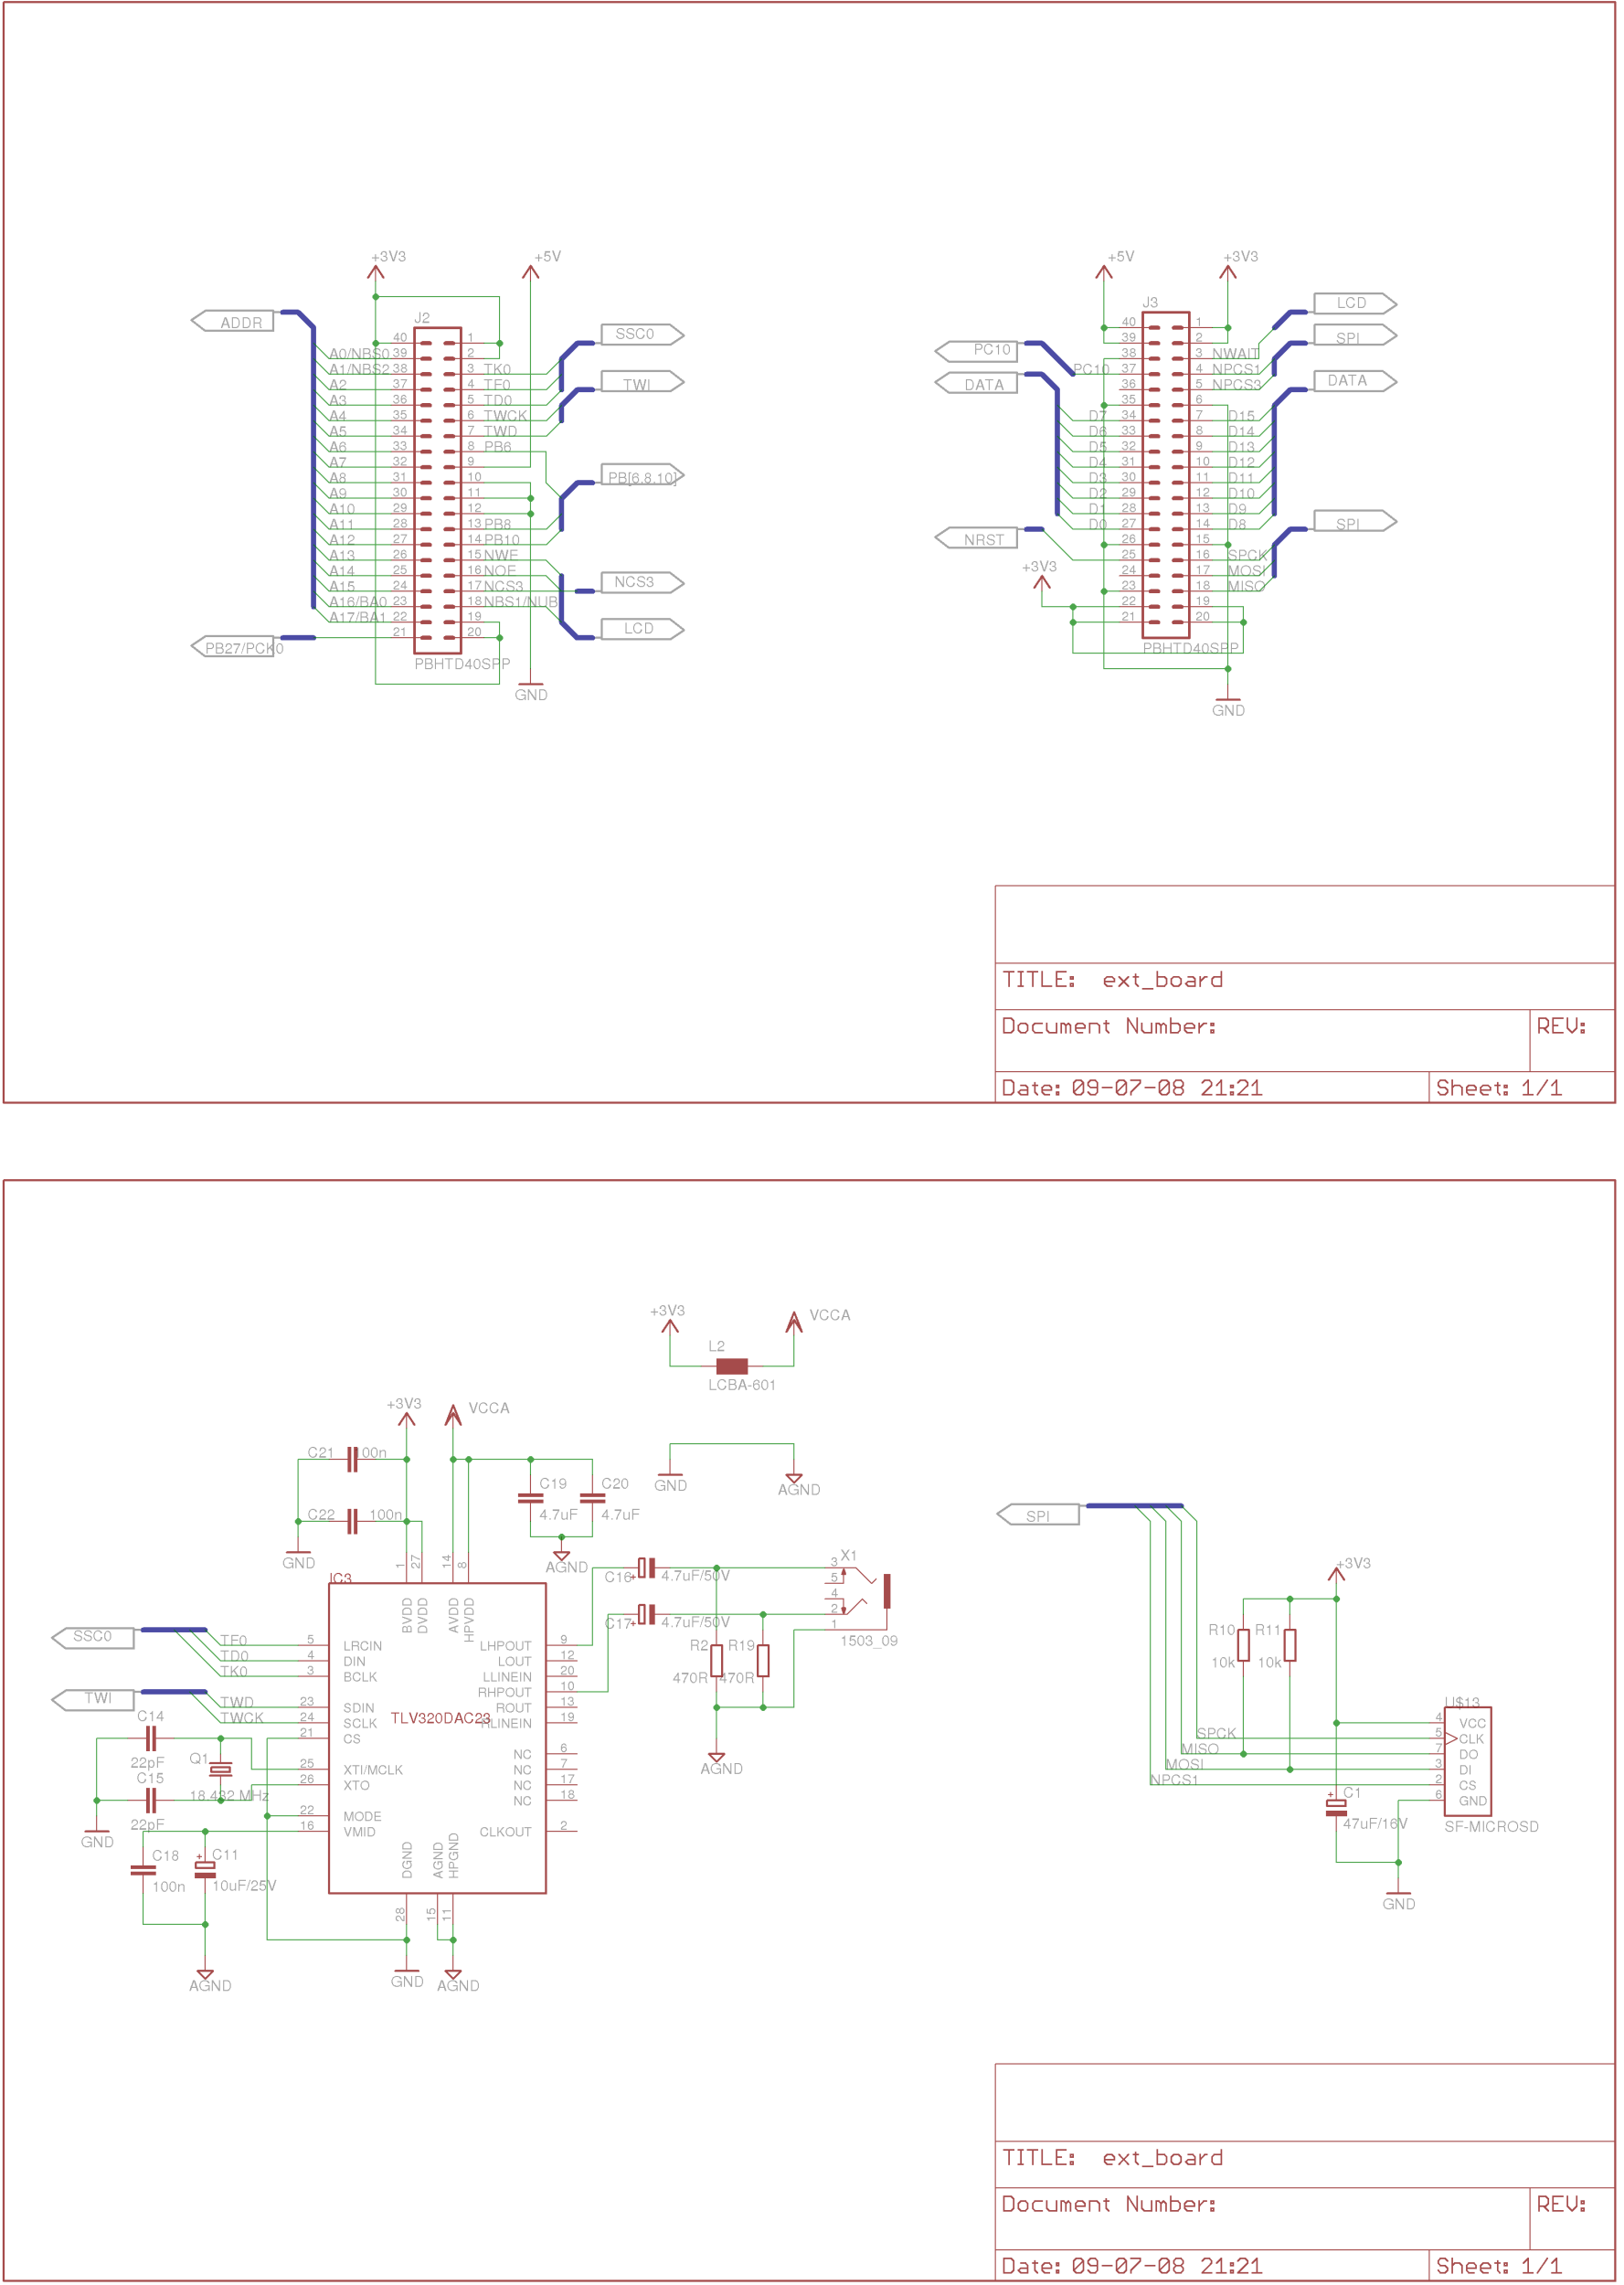
\includegraphics[scale=1.0]{img/ext_sch2.png}
%				\caption{Schemat podłączenia dodatkowych elementów rozszerzających możliwości projektu}
%			\end{center}
%		\end{figure}
%		
%		\begin{figure}[]
%			\begin{center}
%				\label{fig:main_brd}
%				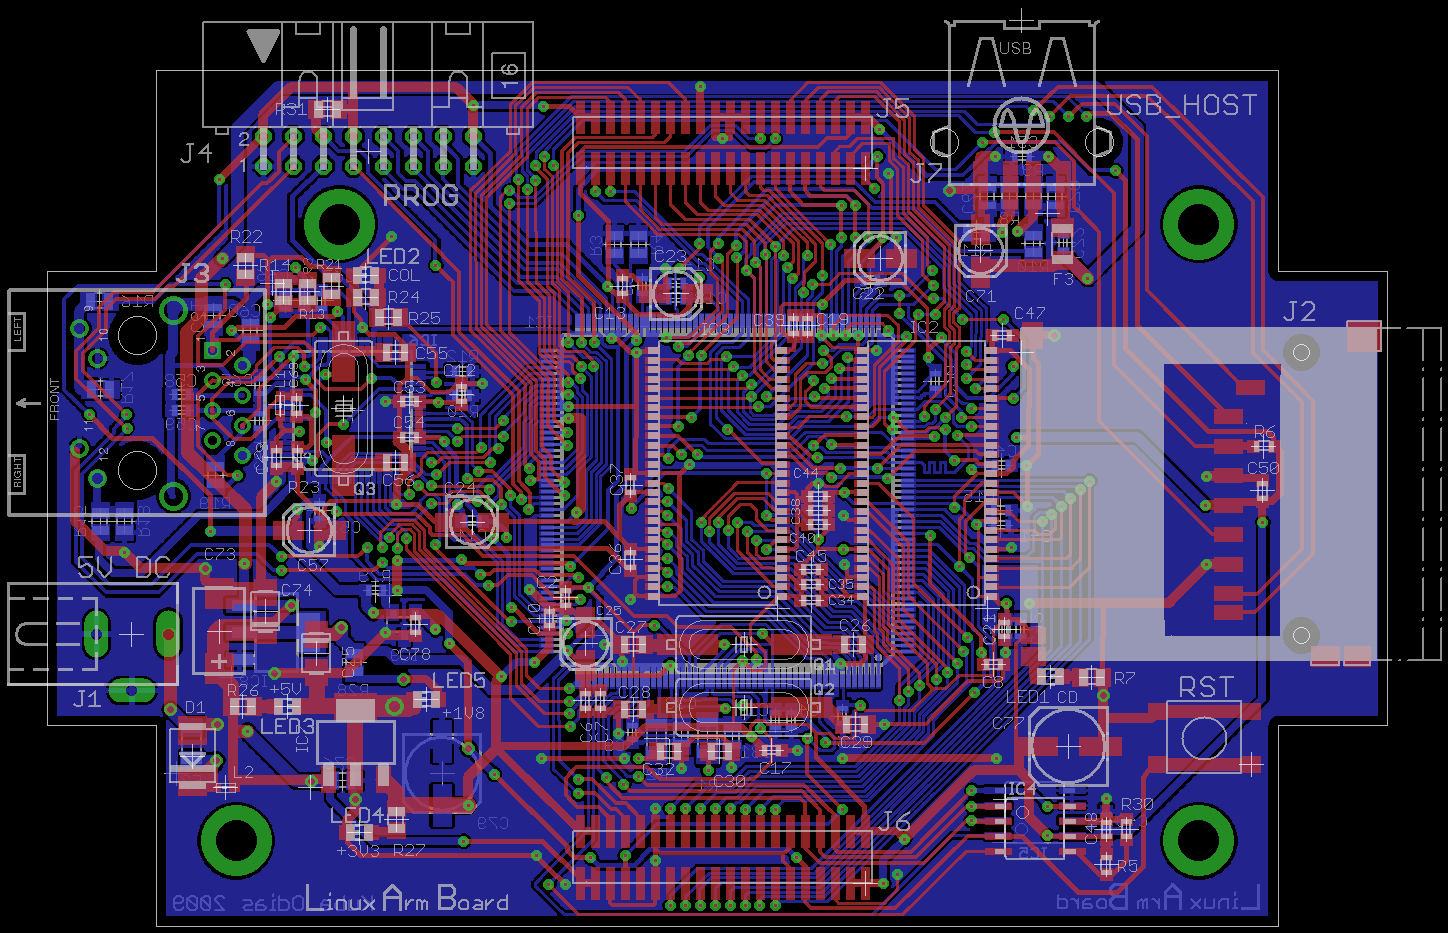
\includegraphics[scale=1.25]{img/main_brd.png}
%				\caption{Plik .brd programu Eagle dla głównej płytki}
%			\end{center}
%		\end{figure}
%		
%		\begin{figure}[]
%			\begin{center}
%				\label{fig:ext_brd}
%				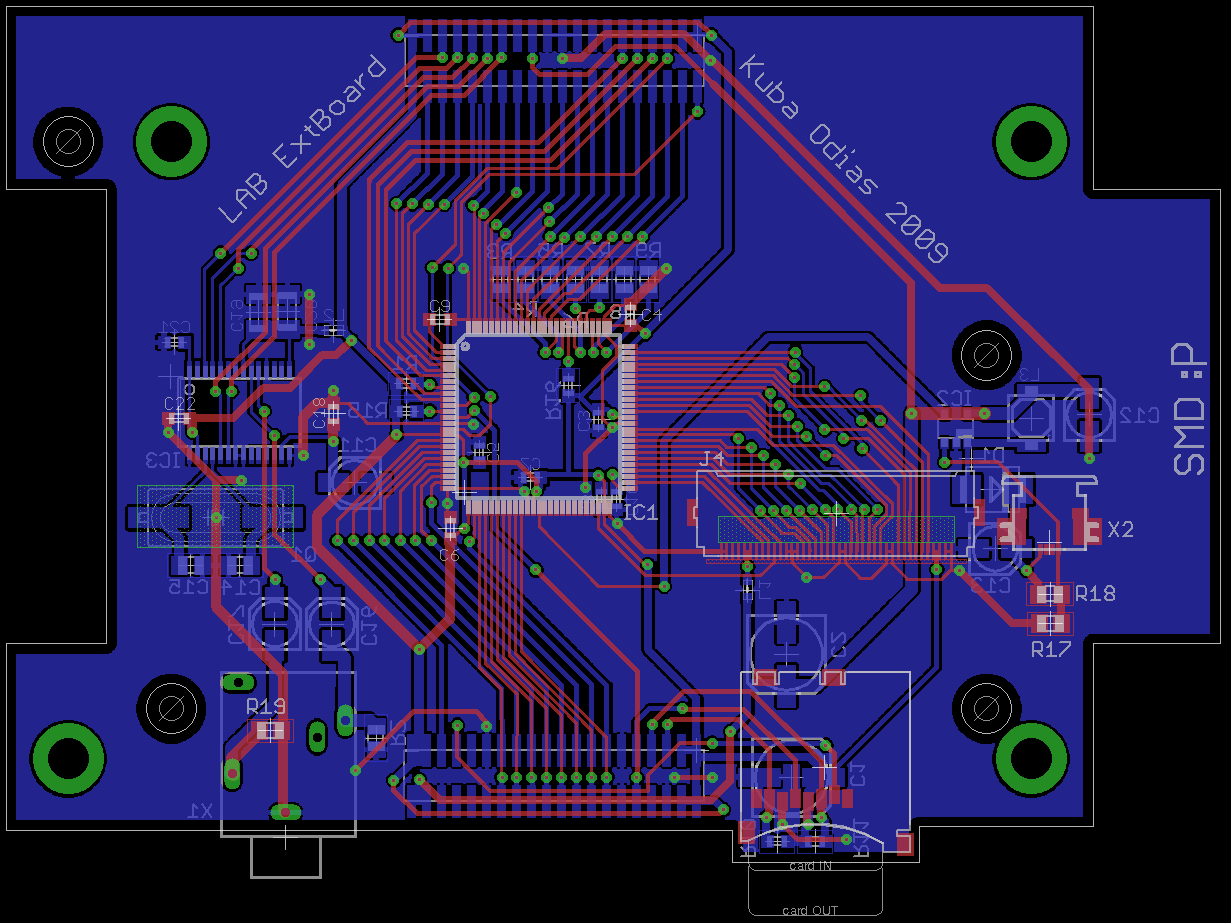
\includegraphics[scale=1.25]{img/ext_brd.png}
%				\caption{Plik .brd programu Eagle dla dodatkowej płytki}
%			\end{center}
%		\end{figure}
%		
%		\begin{figure}[]
%			\begin{center}
%				\subfigure[Górna strona]{\label{fig:pcb1-top}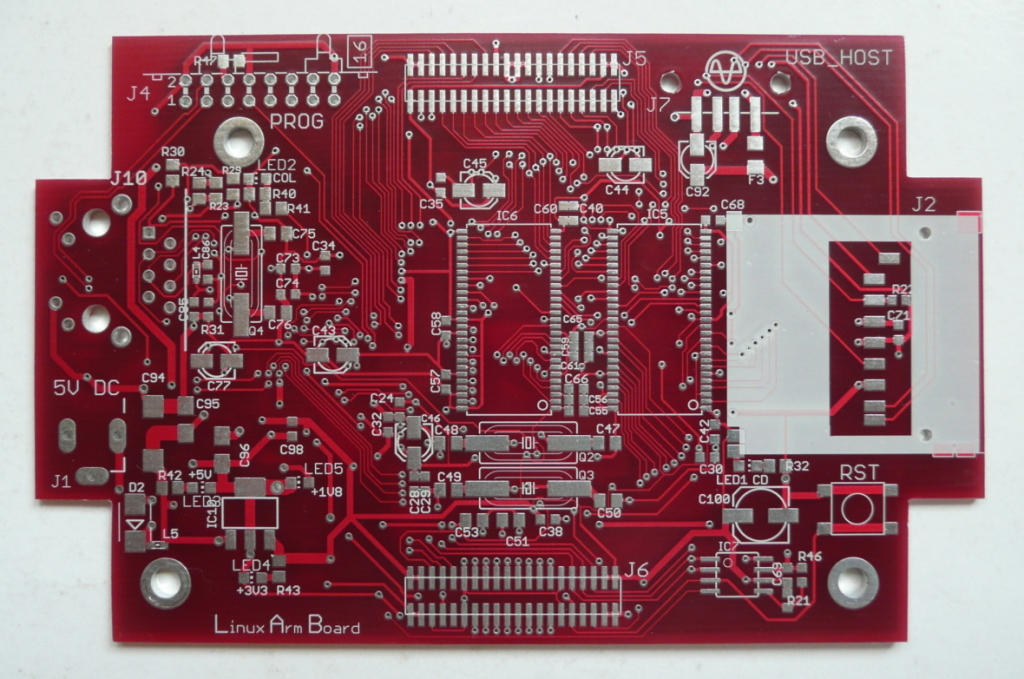
\includegraphics[scale=0.25,angle=90]{img/pcb1_top.jpg}}
%				\hspace{20pt}
%				\subfigure[Dolna strona]{\label{fig:pcb1-bottom}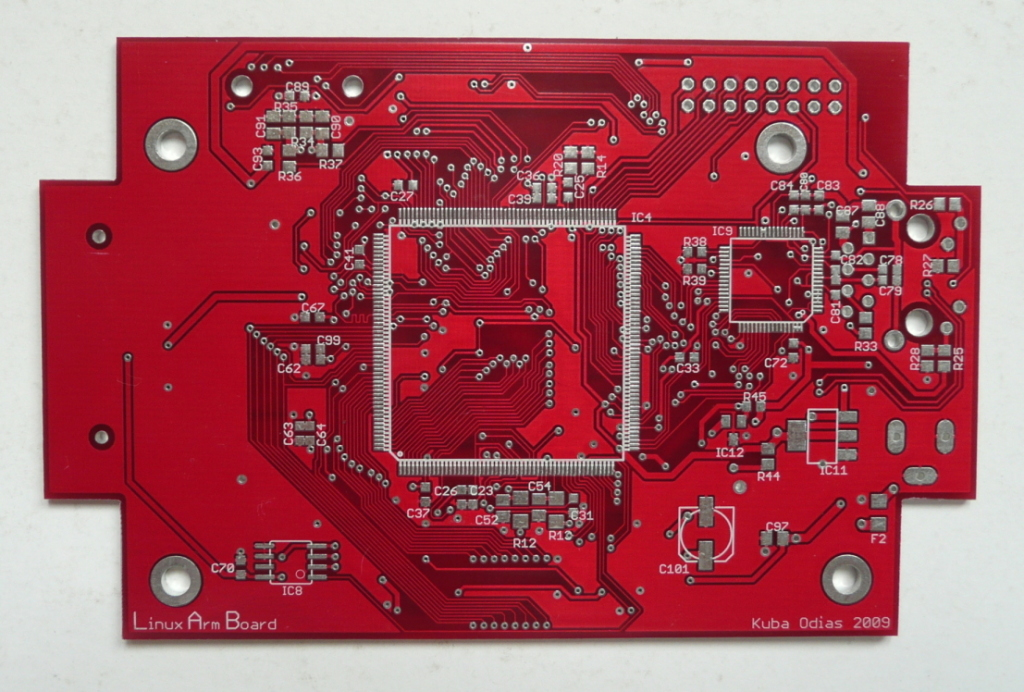
\includegraphics[scale=0.25,angle=90]{img/pcb1_bottom.jpg}}\\
%				\vspace{20pt}
%				\subfigure[Górna strona z przylutowanymi elementami]{\label{fig:pcb1-top}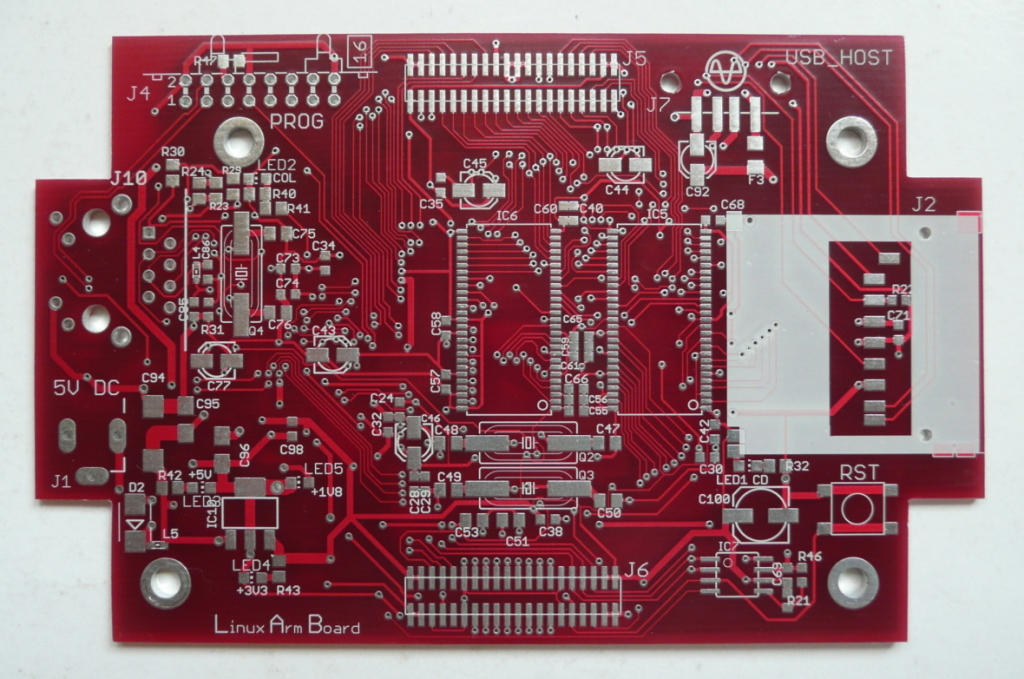
\includegraphics[scale=0.25,angle=90]{img/pcb1_top.jpg}}
%				\hspace{20pt}
%				\subfigure[Dolna strona z przylutowanymi elementami]{\label{fig:pcb1-bottom}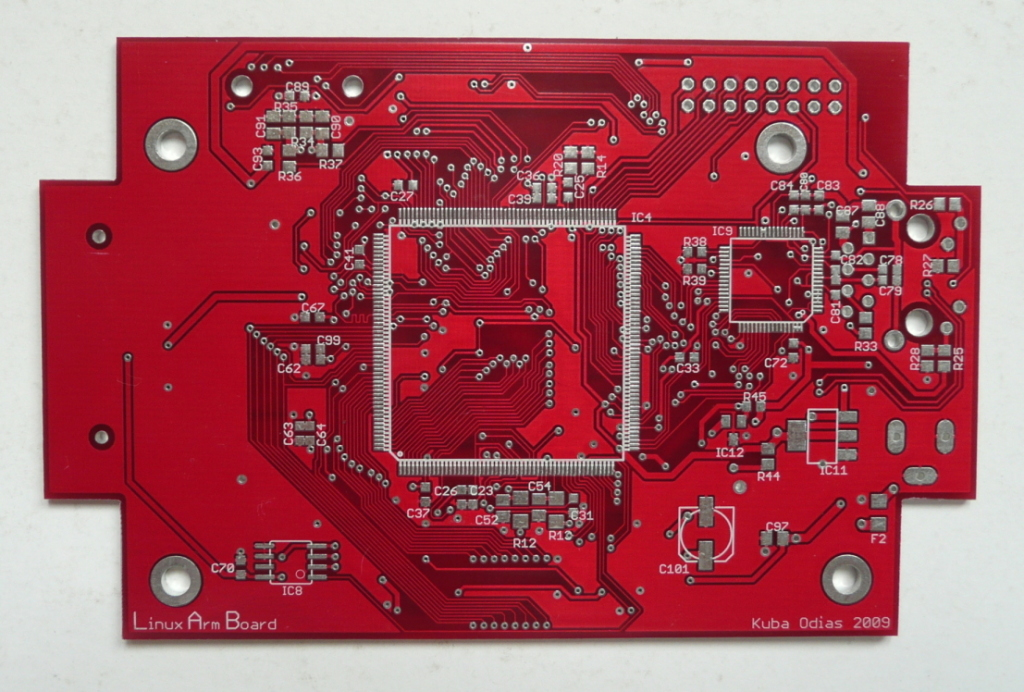
\includegraphics[scale=0.25,angle=90]{img/pcb1_bottom.jpg}}
%			\end{center}
%			\caption{Główna płytka drukowana}
%			\label{fig:pcb1}
%		\end{figure}
%		\begin{figure}[]
%			\begin{center}
%				\subfigure[Górna strona]{\label{fig:pcb2-top}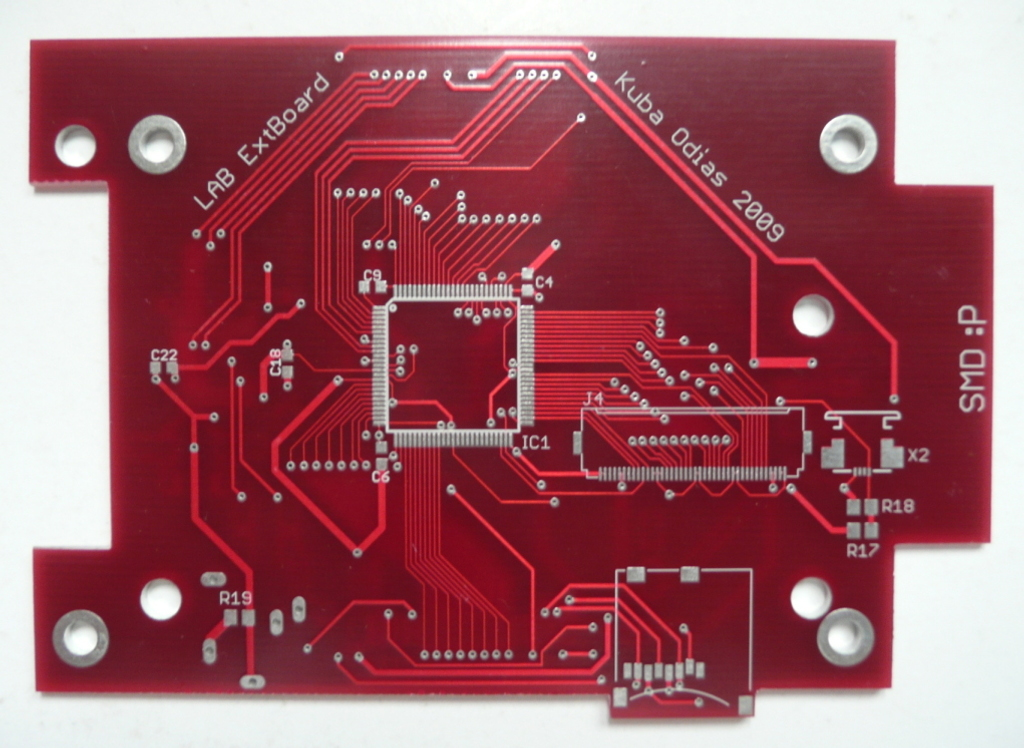
\includegraphics[scale=0.25,angle=90]{img/pcb2_top.jpg}}
%				\hspace{20pt}
%				\subfigure[Dolna strona]{\label{fig:pcb2-bottom}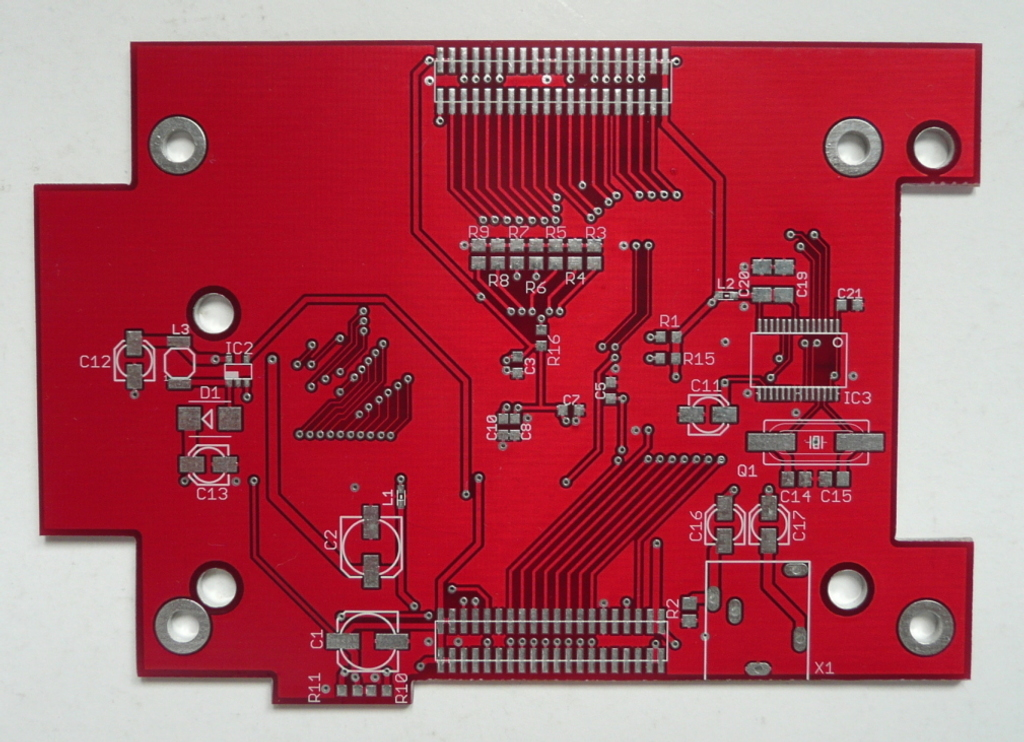
\includegraphics[scale=0.25,angle=90]{img/pcb2_bottom.jpg}}\\
%				\vspace{20pt}
%				\subfigure[Górna strona z przylutowanymi elementami]{\label{fig:pcb2-top}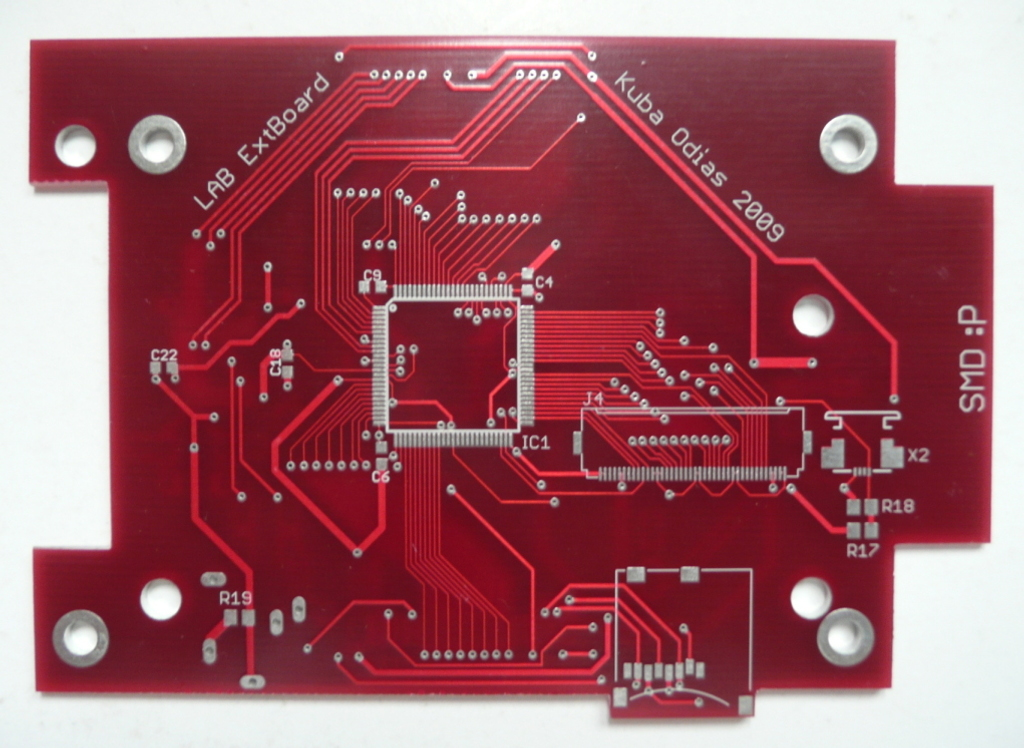
\includegraphics[scale=0.25,angle=90]{img/pcb2_top.jpg}}
%				\hspace{20pt}
%				\subfigure[Dolna strona z przylutowanymi elementami]{\label{fig:pcb2-bottom}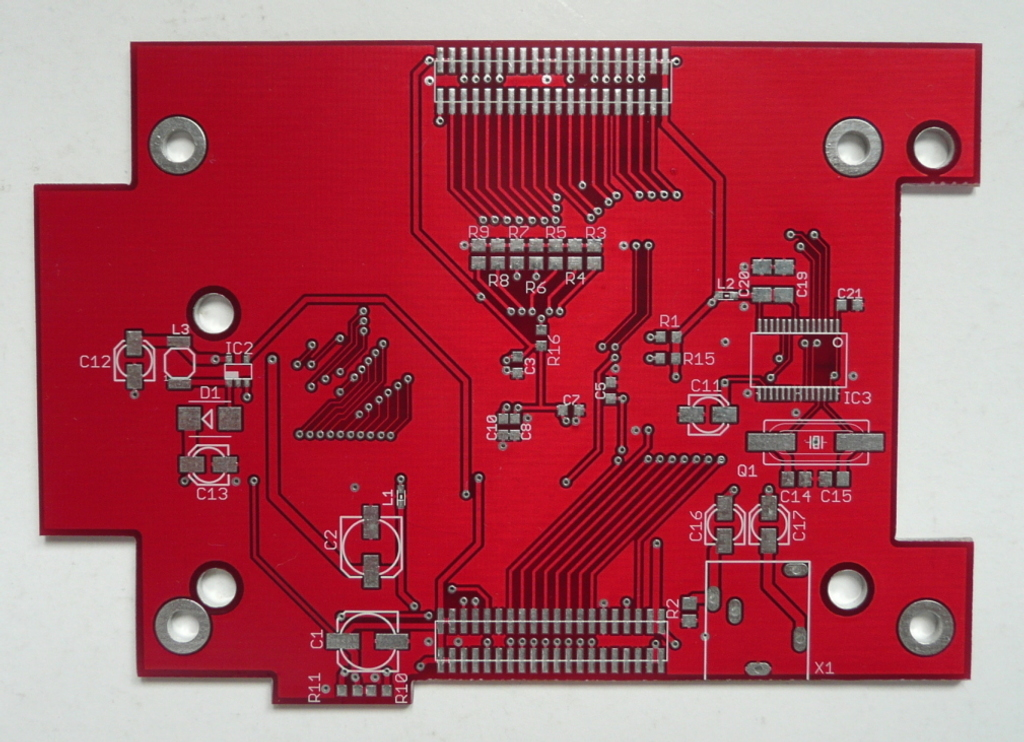
\includegraphics[scale=0.25,angle=90]{img/pcb2_bottom.jpg}}
%			\end{center}
%			\caption{Dodatkowa płytka drukowana}
%			\label{fig:pcb2}
%		\end{figure}
%	
%		\begin{figure}[]
%			\begin{center}
%				\subfigure[Schemat ideowy programatora wykonany w programie Eagle]{\label{fig:programator_sch}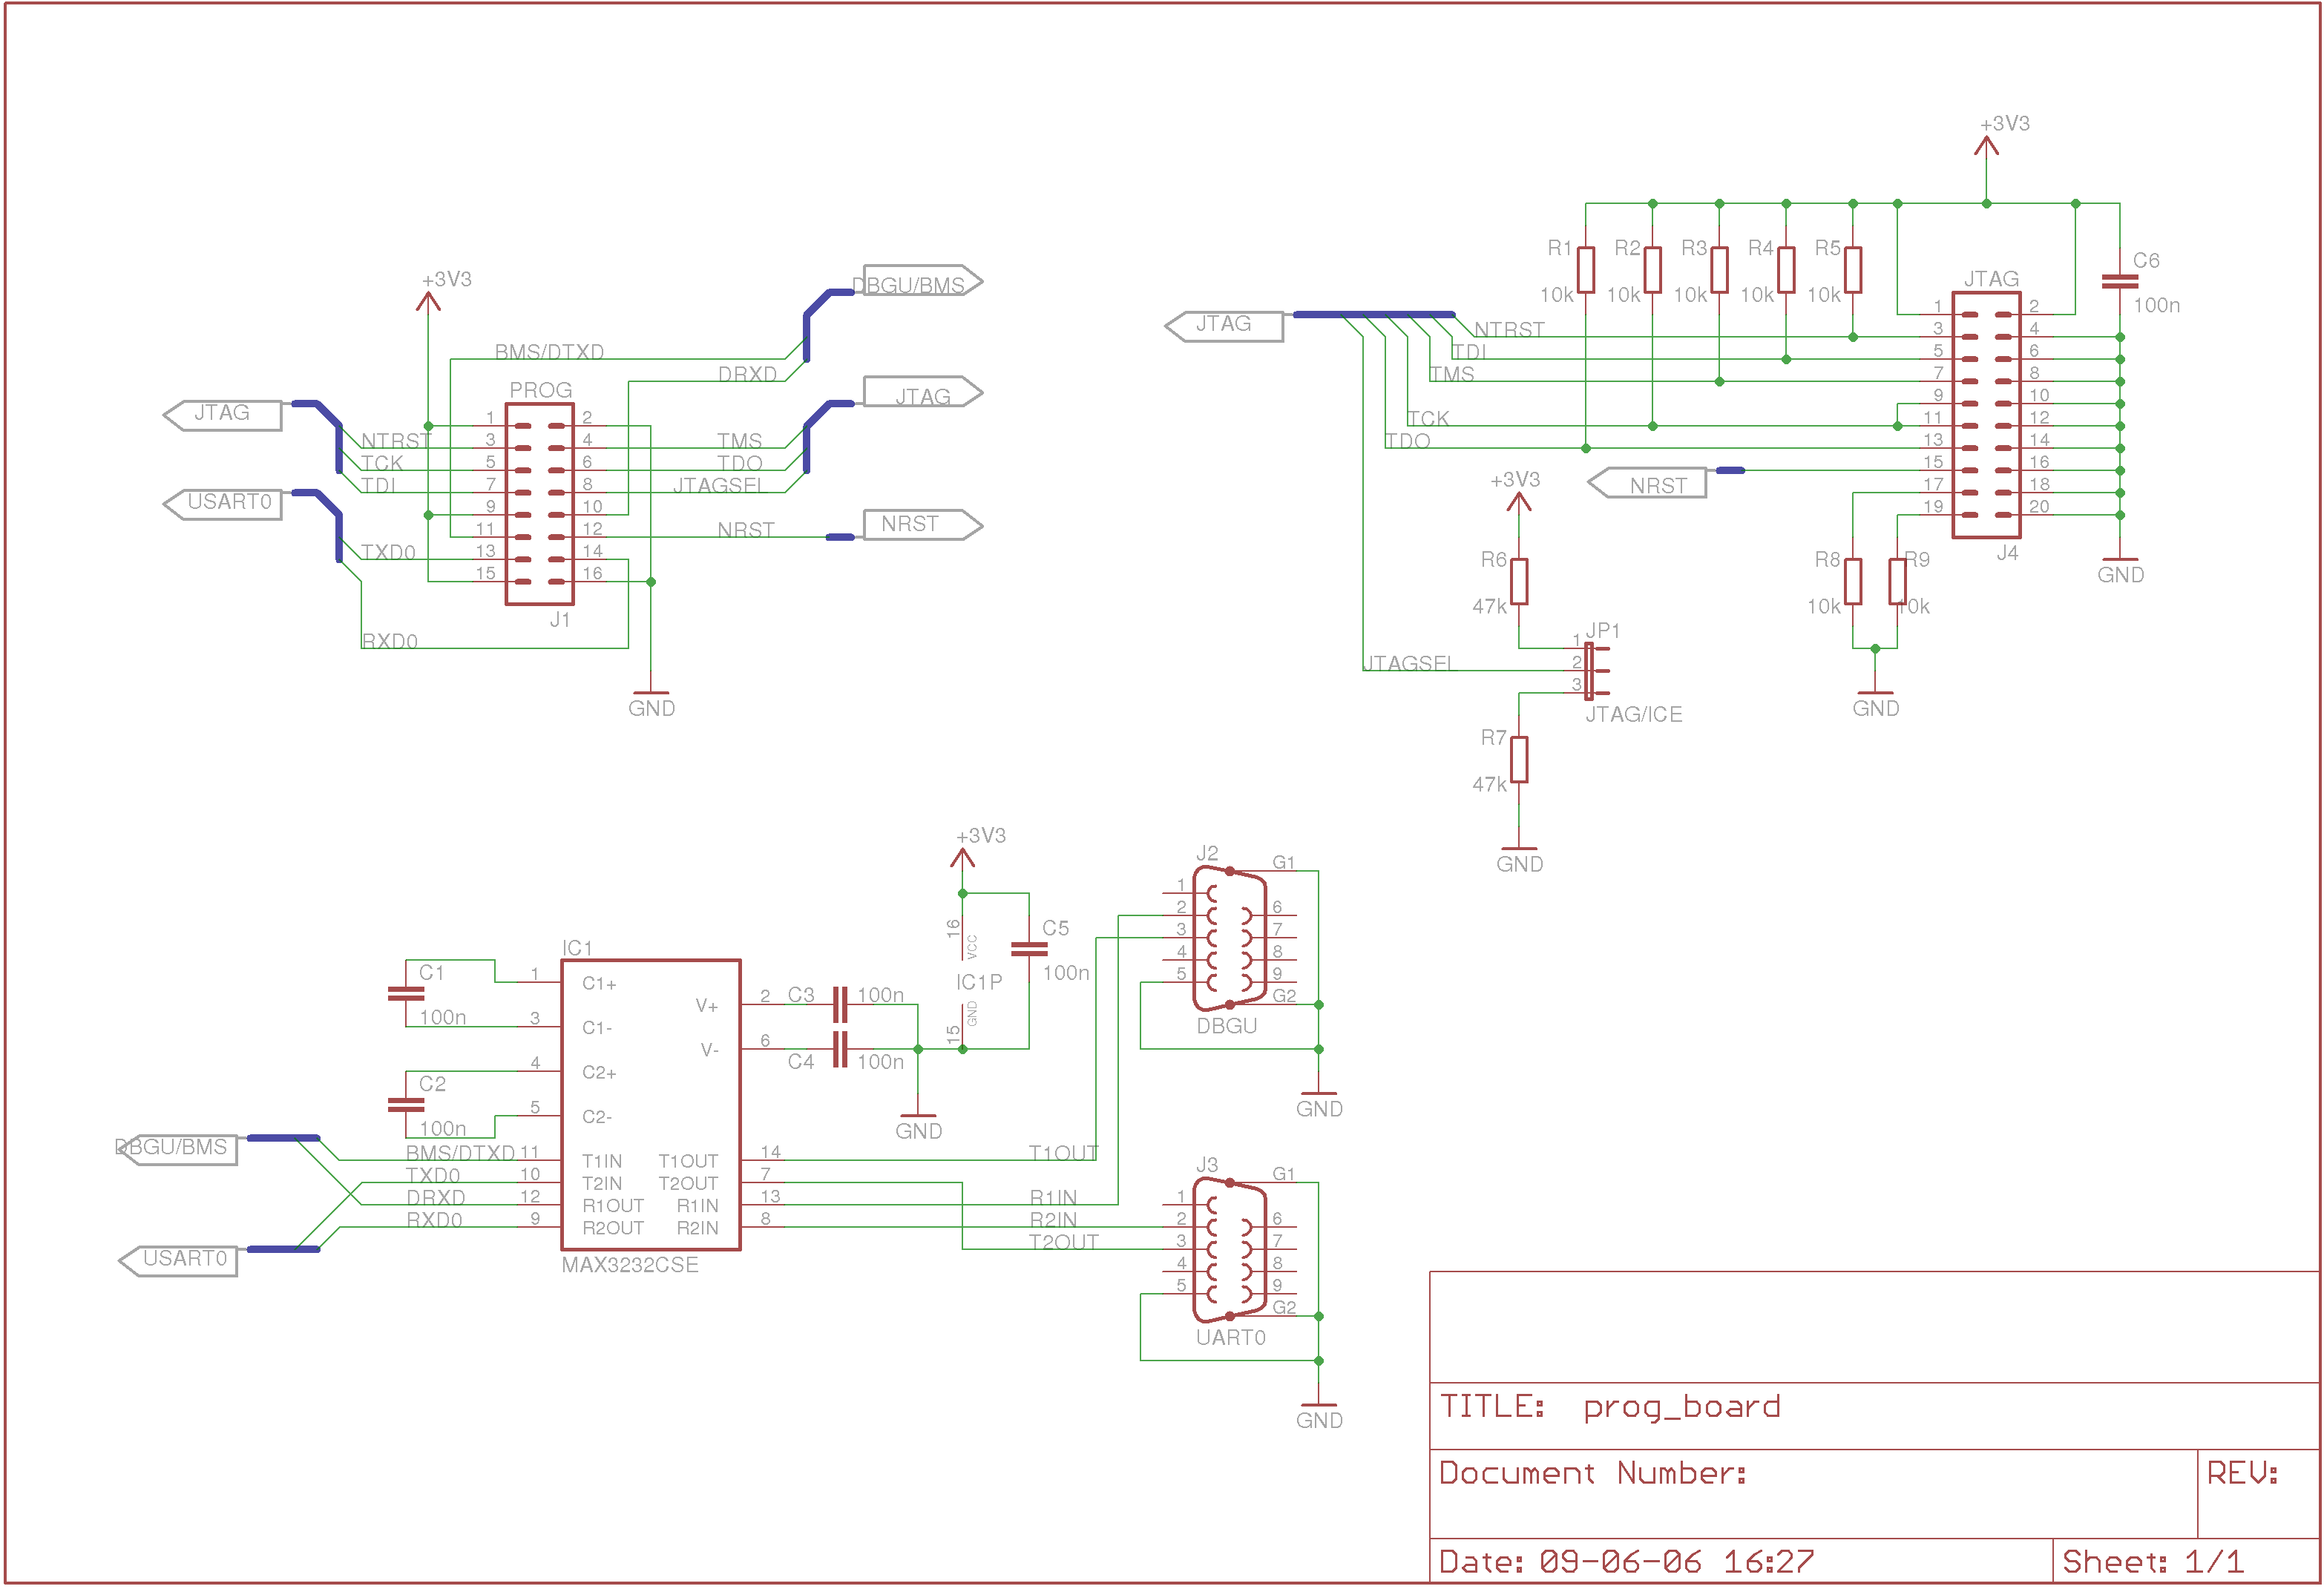
\includegraphics[scale=0.55]{img/programator_sch.png}}\\
%				\vspace{40pt}
%				\subfigure[Plik .brd programu Eagle dla programaora]{\label{fig:programator_brd}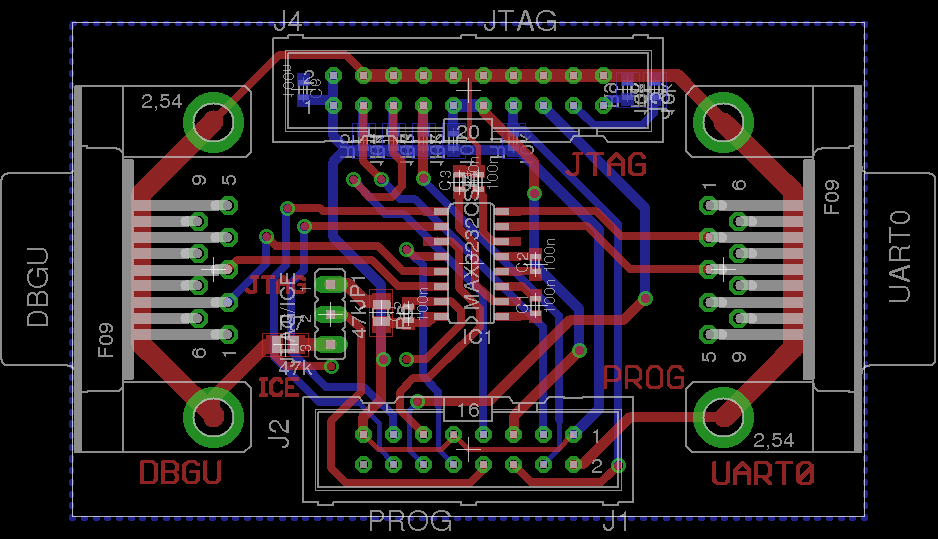
\includegraphics[scale=1.4]{img/programator_brd.png}}
%			\end{center}
%			\caption{Projekt programatora}
%			\label{fig:programator}
%		\end{figure}
%	
	
	\chapter{Przykładowe projekty}
	\label{app:przykladowe_projekty}
	\begin{itemize}
		\item \texttt{http://www.atmel.com/dyn/resources/prod\_documents/doc6103.pdf}\\
			Zestaw uruchomieniowy firmy Atmel dla AT91RM9200.\\
			\scriptsize{(strona odwiedzana w dniu 15.08.2009)}
			\normalsize
		\item \texttt{http://blackmesaeast.com.pl/projects/electronics/sarge-single-\\board-computer/}\\
			Projekt autorstwa Grzegorza Rajtara wykorzystujący mikrokontroler AT91RM9200 i kontroler sieciowy STE100P.\\
			\scriptsize{(strona odwiedzana w dniu 15.08.2009)}
			\normalsize
		\item \texttt{http://bryndza.boff.pl/index.php?dz=proj\&id=armputer210}\\
			Projekt autorstwa Lucjana Bryndzy pełniący rolę serwera sieciowego.\\
			\scriptsize{(strona odwiedzana w dniu 15.08.2009)}
			\normalsize
		\item \texttt{http://www.olimex.com/dev/sam9-L9261.html}\\
			Zestaw uruchomieniowy firmy Olimex dla mikroprocesora AT91SAM9261.\\
			\scriptsize{(strona odwiedzana w dniu 15.08.2009)}
			\normalsize
	\end{itemize}
	
\end{document}